\documentclass[uplatex]{jsarticle}
\usepackage[dvipdfmx]{graphicx}
\usepackage{ascmac}
\usepackage{listings}
\usepackage{amsmath}
\usepackage{bm}
\usepackage{cases}

\DeclareMathOperator*{\minimize}{minimize}

\title{統計的機械学習 2017年夏学期 シケプリ}
\author{@asarihamaguri01}
\begin{document}
\maketitle

\section{はじめに}
2017年度春学期より開講の鶴岡先生による「統計的機械学習」のシケプリです。基本的には授業スライドのまとめ、\
省略されている用語の解説や勾配計算、口頭で説明された内容をまとめています。数式についてはできるだけチェックしていますが、\
もしミスなどあれば教えていただけると嬉しいです。



\section{統計的機械学習の基本}
\subsection{教師あり学習と教師なし学習(第一講)}
統計的機械学習で扱われる問題は教師あり学習」「教師なし学習」、「強化学習」に大別できます。統計的機械学習の授業では教師あり学習、教師なし学習についての扱います。

\begin{itembox}[l]{教師あり学習」と「教師なし学習}
  \begin{description}
    \item [教室き学習(supervised Learning)]\mbox{}\\
    入力から出力を予測するモデルを学習、正解が与えられている。
    \item [教師なし学習(unsupervised learning)]\mbox{}\\
    予測の対象となる出力(正解)が与えられない、データの構造や関係を解析
  \end{description}
\end{itembox}

授業で紹介されたアメリカ東海岸エリアの労働者の賃金データですWage\footnote{https://vincentarelbundock.github.io/Rdatasets/doc/ISLR/Wage.html}は\
それぞれの労働者のage, sex, year, race等の情報と賃金のデータが与えられているため、このデータを用いてモデルを正しく学習させることで年齢や性別等の情報が与えられた時にその人の賃金を予測するモデルを作ることができます。\
このように入力、出力が共に与えられ、入力から出力を予測する回帰、分類等の問題を教師あり学習と言います。

一方、遺伝子の発現データであるNCI60 Data\footnote{https://www.rdocumentation.org/packages/made4/versions/1.46.0/topics/NCI60}は\
特に出力が与えられているわけではなく、データを様々な軸でクラスタリングします。こういった正解ラベルを与えることなく、データからある一定数のクラスに分類する問題は教師なし学習に分類されます。

\subsection{記法について}
まず$p$個の特徴量(年齢、性別など予測を行うために参照できる情報)を持つ$n$個入力データについては、$i$番目の観測データの$j$番目の変数を$x_{ij}$とすると、以下のようなベクトルXで表します。
\[
  \bm{X} = \left(
    \begin{array}{cccc}
      x_{11} & x_{12} & \ldots & x_{1p} \\
      x_{21} & x_{22} & \ldots & x_{2p} \\
      \vdots & \vdots & \ddots & \vdots \\
      x_{n1} & x_{n2} & \ldots & x_{np}
    \end{array}
  \right)
\]
ここで$i$番目の観測データを表すベクトルを$x_i^T = (x_{i1} \ x_{i2} \ \ldots x_{ip})$とすると$\footnote{蛇足かもしれませんがTは行列の転置を意味しています}$以下のように記述することも可能です。
\[
  \bm{X} = \left(
    \begin{array}{c}
      x_1^T \\
      x_2^T\\
      \vdots \\
      x_n^T
    \end{array}
  \right)
\]
一方、予測の対象は何らかのスカラー値で表されます(分類問題の際にはカテゴリの名前等になることもあります)。
\[
  \bm{y} = \left(
    \begin{array}{c}
      x_1 \\
      x_2\\
      \vdots \\
      x_n
    \end{array}
  \right)
\]
観測データはこの入力$X$及び出力$y$のペアで以下のように表されます。
$$\{(x_1, y_1), (x_2, y_2), \ldots (x_n, y_n)\}$$

\subsection{統計的学習とは(第3講)}
統計的学習とは、入力$X = (X_1, X_2, \ldots, X_p)$と出力$Y$の間にある関係が存在すると過程、入力データ$X$からYを推定できることを目指します。
\begin{itembox}[l]{入力と出力}
  \begin{description}
    \item[入力]\mbox{}\\
    統計的機械学習において、予測行うために与えるデータ。AdvertisementデータセットにおけるTV, Radio, newspaperなど。入力変数、予測変数、特徴量(素性)などと呼ばれる。
    \item[出力]\mbox{}\\
    学習されたデータに入力データを与えた時に返される予測結果。出力変数、応答変数、従属変数などど呼ばれる。
  \end{description}
  統計的機械学習では、以上の入力$X = (X_1, X_2, \dots , X_p)$と出力Yの間にある何らかのシステマティックな関係$f$をを予測することを目指す。
  $$Y = f(X) + \varepsilon$$
\end{itembox}

またここで$\varepsilon$は確率的な誤差(error)を示しており平均はゼロになります。

統計的推定はパラメトリックな手法とノンパラメトリックな手法があります。
\begin{itembox}[l]{パラメトリックな手法とノンパラメトリックな手法}
  \begin{description}
    \item [パラメトリックな手法]\mbox{}\\
    $f$の関数形について例えば線形モデルの$f(X) = \beta_0 + \beta_1 X_1$等の過程をあらかじめ置いて置き、\
    学習を通して仮定された関数の係数$\beta_0, \beta_1 \dots \beta_p$を求める。
    \item [ノンパラメトリックな手法]\mbox{}\\
    $f$の関数形について事前に明示的な仮定を置かない手法。
  \end{description}
\end{itembox}
パラメトリックな手法は$f$の推定問題を$p+1$個のパラメータの値を求めるというシンプルなものに帰着できるという利点がある一方、\
仮定されたモデルが真の$f$を表現できるかどうかは事前にはわからず、表現力の高いモデルを仮定すると過学習$\footnote{学習データの中のノイズにも適応し過ぎてしまい、新しい入力に対して正しい予測をできなくなってしまうこと}$が起こってしまう恐れがあります。
ノンパラメトリックな手法は複雑な$f$を表現できる可能性があり、また高精度の推定のためにはパラメトリックモデルよりも大量の観測データが必要になるケースが多いです。\

このように$xとyの間に存在する関数f$を推定する目的としては、予測及び推論という二つの目的があります。
\begin{description}
  \item[目的1 : 予測(prediction)]\mbox{}\\
  Yが容易に得られない場合に、XからYを予測し、推定する。\
  例えば患者に初めての薬を処方する際、その患者が服用して副作用が起こる可能性があるかどうか、事前に予測する必要がる。ここで過去の副作用発生事例から\
  副作用を起こした患者、起こしていない患者の年齢、持病、性別等のデータXより、この新しい患者がある薬に対して重篤な副作用が起きるリスクいう出力$Y$を事前に推定することができる。
  このように予測が目的です時は推定結果が正確です限り、$\hat{f}$はブラックボックス化して構わない。
  \item[目的2 : 推論(inference)]
  $X_1, X_2, \dots , X_p$が変化した時にYがどのように変わるかを知りたい。これはどの入力変数がYに関係しているかを知り、活用することを目指している。\
  例えばAdvertisingデータセットにおける学習では、知りたいのは「何らかのシステマティックな関係により売り上げがいくつかになる」\
  ではなく、例えばTV広告を増やした時、新聞広告を増やした時でどのくらい売り上げが変わるのかを知るため、\
  Yと入力変数Xの間にある線形もしくは非線形な関係を知り、どのXがYに影響を与えているかそのウェイトの大きさをみる。
\end{description}
目的を予測にするか推論にするかにより、選択されるべき適切なモデルは異なってきます。\
例えば推論を目的とするならば、推定した関数の中身の解釈が比較的容易な線形モデルや、どのように条件を分岐させているかを可視化できる決定木モデルなどがどの\
独立変数がどう従属変数に影響を与えているんか容易に確認が可能です。一方線形モデルでは複雑非線形な関係に対応できず、決定機は入力データに左右されるため、\
常に高い精度が得られるわけでありません。予測のみを目的とするならば、対象が複雑な現象であっても高い予測精度が得られる可能性がある非線形モデルが適しているかもしれませんが、\
非線形モデルは中身の解釈が難しく、推論には使いにくい傾向にあります$\footnote{現在でも広く使用されている機械学習モデルの一つにSVM(サポートヴェクターマシン)というものがあり、これは\
非線形な関係にも対応でき一般的なタスクにおいて線形モデルより高い精度を発揮することも多いのですが、線形モデルと比較するとどの入力変数が出力とどの程度影響を与えているか直接知ることはできません。\
また機械学習ではないですが、今話題の深層学習もモデル自体をブラックボックス化してしまい、人間が直接的にどうそれぞれの入力変数が影響を与えているのか知る方法はありません}。$
\begin{itembox}[l]{予測精度と解釈性のトレードオフ}
  \begin{itemize}
    \item 表現力の低いモデルでは複雑な形の$f$をうまく近似できない一方、 $Y$と$X_1, X_2 \dots X_p$の関係がわかりやすい。(予測精度は低いが解釈性が高い)
    \item 表現力の高いモデルでは多様な$f$に対応が可能ですが、$Y$と$X_1, X_2 \dots X_p$の関係がわかりづらい。(予測精度は高いが解釈性が低い)
  \end{itemize}
\end{itembox}
% 以下のグラフは様々なグラフの予測精度と解釈性について配置したものであり、
% \begin{figure}
%   \begin{center}
%     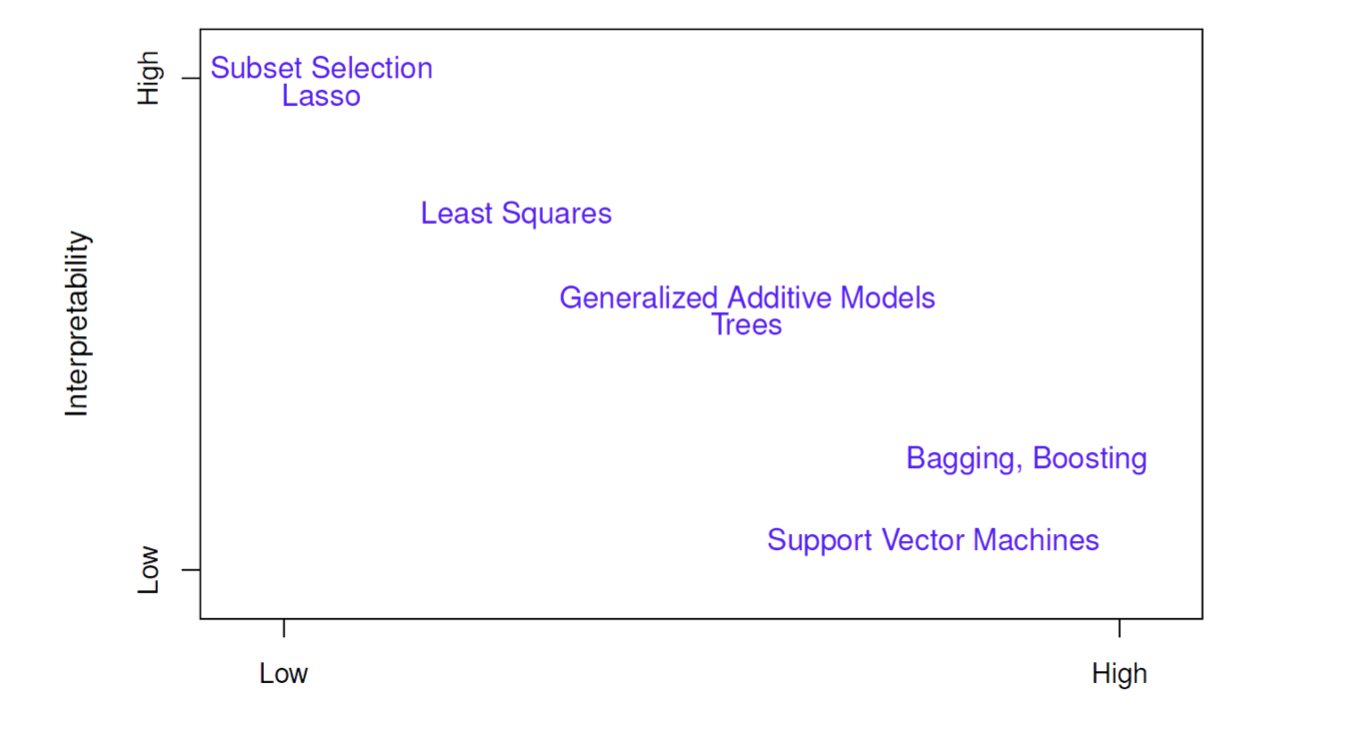
\includegraphics[width=13cm]{img/tradeoff.png}
%     \caption{予測精度と解釈性}
%   \end{center}
% \end{figure}
% 実際に解釈性が高いモデルは予測精度が低く、解釈性の低いモデルは予測精度が高く出ることがわかります。

\section{回帰と分類(第3講)}
\subsection{変数の種類}
統計的機械学習ではある一つ以上の入力変数$X$から、出力$y$を推定する$f$を求めことを目的としますが、入力変数$X$には連続した実数値となる量的変数と、\
離散的なカテゴリ(ラベル)になる質的変数があります。
\begin{itembox}[l]{量的変数と質的変数}
  \begin{description}
    \item [量的変数]\mbox{}\\
    年齢、身長、収入、株価などの連続的な実数値をとる変数。そのまま入力変数として使用することができる。
    \item [質的変数]\mbox{}\\
    性別、学歴、Yes/No、カテゴリの種類など、$K$個の異なるクラス(カテゴリ)からどれかの値をとる変数。そのままでは入力変数として用いることができず、\
    後述するダミー変数の使用などにより予測モデルに組み込む。
  \end{description}
\end{itembox}
教師あり学習は回帰問題と分類問題に大別することができ、回帰問題(regression Problem)では予測変数が金融商品の価格等の量的変数となる一方、\
分類問題(classification problem)では予測対象が債務不履行に陥ったか否かなどの質的変数になります。\\

補足ですが、質的変数を入力変数として用いた予測モデルを作る際には「女性/男性」などの情報はそのままでは数理モデルに組み込むことができないのでそれぞれの質的変数(質的変数に含まれるカテゴリ)ごとにダミー変数を作成することが一般的です。\
例えば「女性/男性」「大人(18歳以上)/子供(18歳未満)」等ある質的変数について完全に2値で分けられるときには以下のように「女性であれば1/男性であれば2」等のように変数を作ります。\\
\[
  x^{gender}_i = \begin{cases}
    1 & ({\rm if\ ith\ person\ is\ a\ female}) \\
    0 & ({\rm if\ ith\ person\ is\ a\ male})
  \end{cases}
\]
ではこのように「true/false」の2値で分類できない場合はどうするのでしょうか。例えばethnicity(民族)について、とりあえずCaucasian = 2, African American = 1, or Asian = 0とか\
適当に数字を振ってしまったら$\footnote{どっかの団体に怒られそうな例だ...}$もともと順序や序列の存在しないデータに恣意的に大小関係を加えることになり、モデルの予測を歪めてしまいかねません。\
そこでこういった複数の値を取りうる質的変数についてはその全てに対してダミー変数を作り、「Asianならば1、そうでければ0」といった風に数字を割り当てます。
\[
  x^{asian}_i = \begin{cases}
    1 & ({\rm if\ ith\ person\ is\ an\ Asian}) \\
    0 & ({\rm if\ ith\ person\ is\ not\ an\ Asian})
  \end{cases}
\]


\subsection{モデルの精度}
モデルの精度の測り方には様々な方法がありますが、回帰問題の場合、平均二乗誤差(mean squared error, MSE)を、分類問題の場合error rateを用いることが一般的です。
\begin{itembox}[l]{平均二乗誤差及びerror rate}
    \begin{description}
      \item [平均二乗誤差(MSE)]\mbox{}\\
      平均二乗誤差とは$n個の$学習データから構築されたモデルの予測した結果と実際のラベルと差を二乗し、平均を撮ったものであり、以下の式で表される。
      $${\rm MSE} = \frac{1}{n}\sum_{i=1}^n (y_i - \hat{f}(x_i))^2$$
      \item [誤り率(error rate)]\mbox{}\\
      error rateは$n$個の学習データに対する予測のうち、誤った予測を行ってしまった数をデータの総数$n$で割ったもの。
      $${\rm error\ rate} = \frac{1}{n}\sum_{i=1}^n I(y_i \neq \hat{y}_i)$$
      ここで$I(y_i \neq \hat{y}_i)$は$y_i \neq \hat{y}_i$ならば1を、そうでなければ0(すなわち正解していれば0)をとる関数。
    \end{description}
\end{itembox}
ちなみにこの式で表されるのは学習データでの誤差(training MSE)ですが、本当に最小化したいのは未知データでの誤差(test MSE)です。気をつけなくてはいけないのは、特に過学習をしている場合などは学習データにおけるMSEがいくら高くても\
Test MSEが必ずしも少なくなっているとは限りません。
$${\rm Ave}((y_0 - \hat{f}(x_0))^2)$$
error rateも同様に上の式で得られるのは学習データでのerror rateに過ぎず以下の式で表されるTest error rateを下げる必要があります。
$${\rm Ave}(I(y_i \neq \hat{y}_i)^2)$$

またモデルの精度を測る指標としてバリアンス(variance)とバイアス(bias)があり、テストMSEはこれらバリアンス及びバイアスで表すことができる。
\begin{itembox}[l]{バリアンスとバイアス}
  \begin{description}
    \item [バリアンス]\mbox{}\\
    学習データの違いによってどれだけモデルによって予測される$\hat{f}$の値が変わるかを示す。未知のデータに対してどのくらい正しく予測できているかを測る。
    \item [バイアス]\mbox{}\\
    真のラベル$f$と予測した値$\hat{f}$がどれだけずれているかを示す。学習データに対して、どのくらい正しく予測できているかを測る。
  \end{description}
\end{itembox}
平滑化スプライン等の表現力の高いモデルは、学習モデルに対しては\
高い精度で予測できる一方、学習データにオーバーフィットしやすく新しい未知データに対して正しく予測できない可能性が高まるため、バリアンスが高い。\
一方線形回帰などの表現力のあまり高くないシンプルなモデルは、このようなオーバーフィットをしにくく、バリアンスは小さくなる傾向にあるが、学習データに対してフィットしきれずバイアスが大きくなります。
このように、バイアスとバリアンスの間にあるトレードオフの関係をThe bias-variance trade-offと言います。
\begin{itembox}[l]{The bias-variance trade-off}
  テストMSEは以下の3つの項の和に分解でき、バイアスとバリアンスにはトレードオフの関係にあることが確認できる。(この導出については参考資料に)
  \begin{itemize}
    \item $\hat{f}(x_0)$のバリアンス(分散)
    \item $\hat{f}(x_0)$のバイアスの二乗
    \item $\varepsilon$の分散
  \end{itemize}
  $${\rm Test MSE} = E[(y_0 - \hat{f}(x_0))^2] = {\rm Var}(\hat{f}(x_0)) + [{\rm Bias (\hat{f}(x_0))}]^2 + {\rm Var}(\varepsilon)$$
\end{itembox}
このバイアスバリアンストレードオフはよく出てくるので正しく答えられるようにしましょう。

\subsection{ベイズ分類器}
条件付き確率が最大になるようなクラスにあるデータ$X_i$を分類する方法です。ベイズ最適決定とも呼ばれます。
\begin{itembox}[l]{ベイズ分類器}
  以下の条件つき確率が最大になるクラスを選び、期待誤り率を最小になることを目指した。
  $$P(Y = j|X = x_0)$$
  ベイズ分類器の誤り率はベイズ誤り率(Bayes error rate)と呼ばれ、以下の式で表される。\
  $$1 - E[{\rm max P_r}(Y = j|X)]$$
  これは回帰問題での削減不可能な誤差に相当している。
\end{itembox}
しかし実際のところ、条件付き確率を正しく知ることはできないので、これはあくまでも理論上の分類器になります。\
ベイズ分類器で分類された結果に基づいてデータの間に惹かれた教会のことをベイズ決定境界といいます。
ベイズ分類器とは頃なる方法で分類を行うことを目指すのが次のK最近傍法です。

\subsection{K最近傍法(K nearest meighbors method)}
K最近傍法は入力変数からそれぞれの入力が属するクラスを予測する分類問題をとくモデルの一つであり、自分に最も近い上位$K$個の観測データの属するカテゴリで多数決を行い、\
自身の最近傍$K$個の観測データの中で最も多く現れたラベルをその入力データのラベルとします。これを定式化すると以下のようになります。
\begin{itembox}[l]{k最近傍法}
  クラスの条件付き確率を以下のように推定し、この確率が最も大きくなったクラスに分類する。
    $$P_r(Y = j|X = x_0) = \frac{1}{K}\sum_{i \in N_0} I(y_i = j)$$
\end{itembox}
この$K$の値を小さく、例えば$K = 1$などにすると、それぞれ自身に最も近い観測データのみ考慮するため、決定境界はより入り組んだ、表現力の高いモデルになります。この場合学習データに対しては高い精度を誇るものの、\
テストデータでは謝り率が高くなることがあ理、モデルの表現力は高すぎても低すぎても、テストエラーが高くなってしまうことに注意が必要です。
KNNで求められたラベルに基づいてデータ間に引かれた境界線がKNN決定境界になります。\
図2の例では$K=1の場合とK=100$の場合のKNN決定境界を見ると、実際にKの数が小さいほど境界線が入り組んでいる、つまり表現力が高くなっていることがわかります。\
この例ではK=1のケースの方がわずかにK=100よりも高いテスト誤り率になってはいますが、図2のKの数に対する学習誤り率とテスト誤り率の推移を見ると、モデルの表現力が高いからといってテスト謝り率は必ずしも下がるわけではないことが確認できます。\
\begin{figure}[htbp]
\begin{minipage}{0.7\hsize}
 \begin{center}
  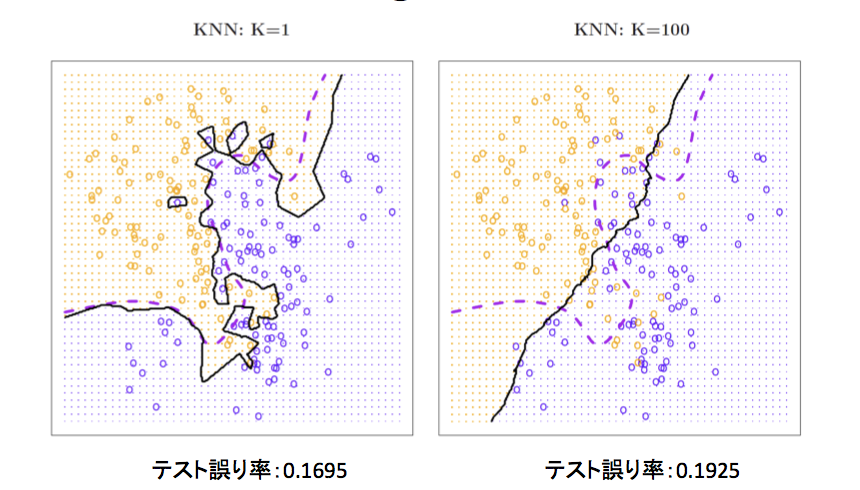
\includegraphics[width=100mm]{img/knn_knum.png}
 \end{center}
 \caption{K=1及びK=100の時のKNN決定境界(黒太線)}
 \label{fig:one}
\end{minipage}
\begin{minipage}{0.3\hsize}
 \begin{center}
  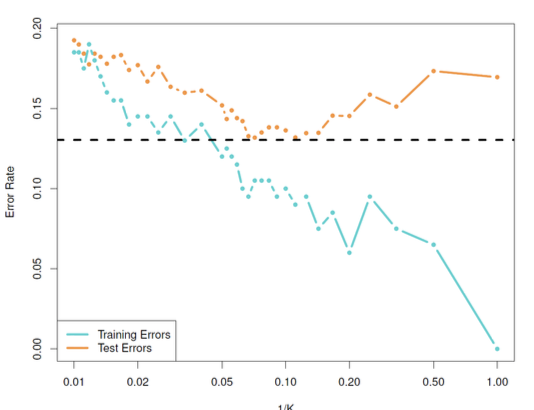
\includegraphics[width=50mm]{img/knn_eror.png}
 \end{center}
 \caption{Kの数に対する学習誤り率とテスト誤り率の推移}
 \label{fig:two}
\end{minipage}
\end{figure}

\subsection{線形回帰(Linear regression)}
\subsubsection{線形単回帰}
線形単回帰とは、$XとY$の関係は線形ですと仮定して、一つの予測変数$X$によって量的応答変数$Y$を予測する。
\begin{itembox}[l]{線形単回帰}
  XとYの関係は以下の式のような線形で表されると仮定する。
    $$Y \approx \beta_0 + \beta_1X$$
    学友データによって適切なパラメータを予測し、$\hat{y} = \hat{\beta_0} + \hat{\beta_1}x$をより元の学習データの結果と近づけることを目指す。
    学習データを${(x_1, y_1), (x_2, y_2), ..., (x_n, y_n)}$とし、予測のずれを残差$e_i = y_i - \hat{y_i}$とすると、線形単回帰の目的関数は以下のように表される。
    $${\rm RSS(残差平方和)} = e_1^2 + e_2 ^2 + e_3^2 + \ldots e_n^2 = (y_1 - \hat{\beta_0} - \hat{\beta_1}x_1)^2 +  (y_2 - \hat{\beta_0} - \hat{\beta_1}x_2)^2 \ldots$$
\end{itembox}
ここで{\rm RSS}は学習データ$X$に対して推定されたパラメータ$\hat{\beta_0}及び\hat{\beta_1}$を用いて線形のモデルで予測した$\hat{y}$の値が、実際の$y$との距離を二乗したものの和であり、\
これを最小化することによりよりずれの少ないモデルを構築することができます。すなわち、線形単回帰においてパラメータを推定するときは残差平方和が最小になるようにパラメータを推定すればいいことになります。\
目的関数${\rm RSS}$を最小化するには、${\rm RSS}$を$\hat{\beta_0}及び\hat{\beta_1}$で微分した時に、それが0なるような$\hat{\beta_0}及び\hat{\beta_1}$を求めれば良いため
$$\frac{\partial {\rm RSS}}{\partial \hat{\beta_0}} = 0, \frac{\partial {\rm RSS}}{\partial \hat{\beta_1}} = 0$$を満たす$\hat{\beta_0}及び\hat{\beta_1}$を求めると、以下のようになります。(詳細な変形などは参考資料に)\\
$$\hat{\beta_1} = \frac{\sum_{i=1}^n (x_i - \overline{x})(y_i - \overline{y})}{\sum_{i=1}^n (x_i - \overline{x})^2}, \hat{beta_0} = \overline{y} - \hat{\beta_1}\overline{x}$$
ここで$\overline{x} = \frac{1}{n}\sum_{i-1}^n x_i, \overline{y} = \frac{1}{n}\sum_{i-1}^n y_i$です。
この結果求められた二つのパラメータ$\hat{\beta_0}, \hat{\beta_1}$がどの程度正確なのかは母回帰直線を推定することにより求めることができます。

\subsubsection{残差{\rm RSS}に関する性質}
また、{\rm RSS}を最小にする$\beta_0, \beta_1$の導出より、以下の二つの性質が求められます。(導出は参考資料に)
\begin{equation}
  \sum_{i=1}^n e_i = 0
\end{equation}
\begin{equation}
  \sum_{i=1}^n e_ix_i = 0
\end{equation}
式(1)は残差の合計が0であることを、式(2)は残差$e_i$と入力$x$はベクトルとして直行であることを意味しています$\footnote{ベクトル a,b の内積がゼロですとき二つのベクトルは直行しているため。}$。

\subsubsection{線形単回帰の信頼性}
線形単回帰においては、母集団において$X, Y$の間に線形の関係性があると仮定しデータよりそのパラメータ$\hat{\beta}_0, \hat{\beta}_1$を予測しており、本来的に母集団の$\beta_0, \beta_1$を予測することはできません。\
そこでデータより得られたパラメータがその程度信頼できるのかを確認します。\
母集団でのXとYの関係を$Y = \beta_0 + \beta_1X + \varepsilon$とすると、$\varepsilon$は母集団における統計的な誤差なので、母集団での回帰直線は$Y=\beta_0 + \beta_1X$であらわsれる。\
以下のように、$Y = 2 + 3X + \varepsilon$という線形の関係を元に生成した人工データに対する線形単回帰モデルに基づくパラメータ推定の結果は以下のようなグラフとなり、実際の母回帰直線と最小二乗による回帰直線の結果にややずれがあることがわかります。\
また与えられた入力データにおける誤差項により異なる観測データに対する最小二乗回帰直線にはややズレがあることが図4 右図よりわかります。
\begin{figure}
  \begin{center}
    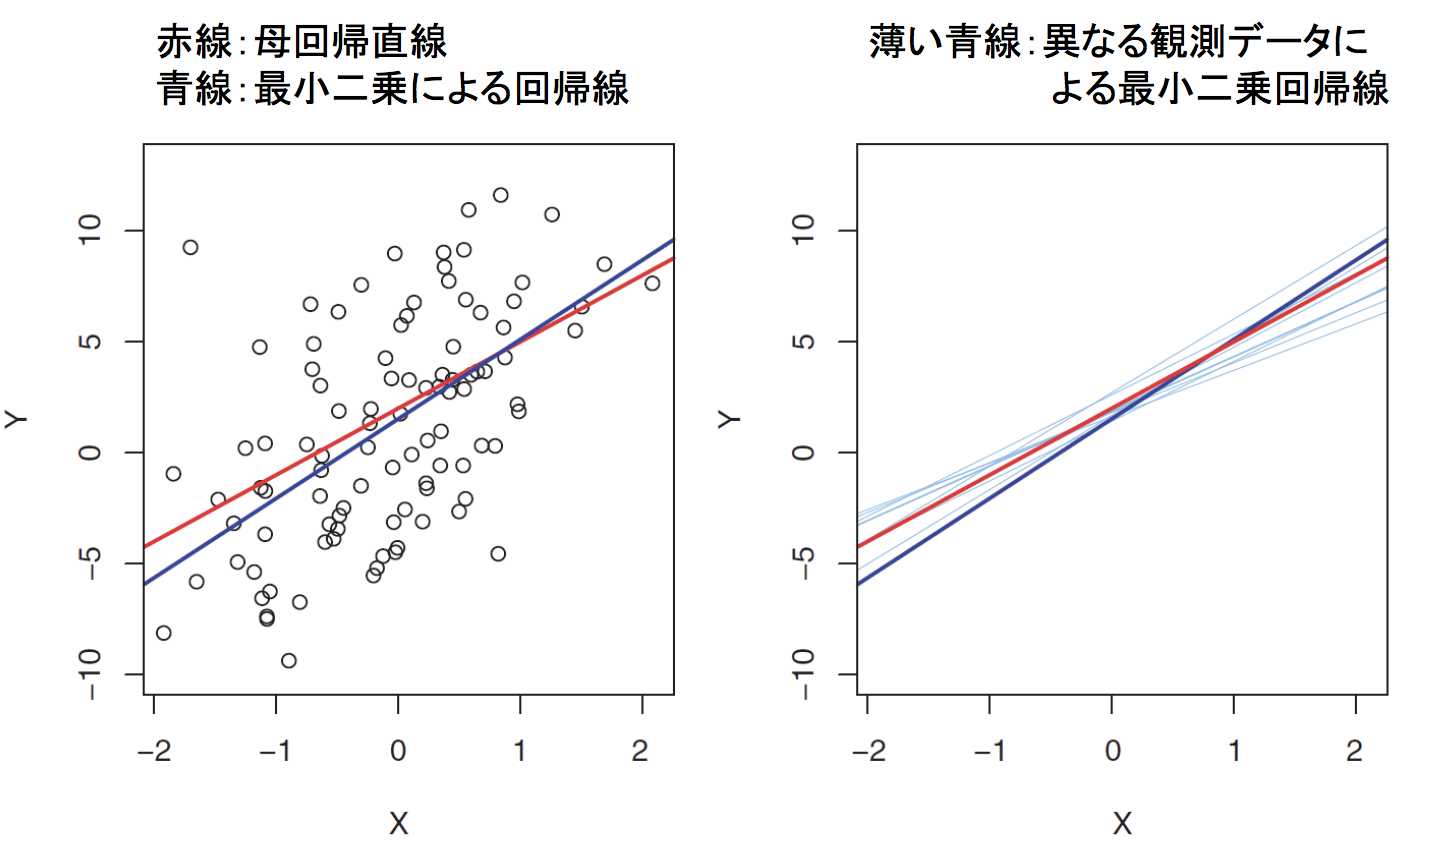
\includegraphics[width=13cm]{img/lienar_error.png}
    \caption{線形単回帰誤差}
  \end{center}
\end{figure}
では求められたパラメータより基礎統計や数理手法でやったように信頼区間を求めるにはどうしたらいいのでしょうか。そのためにまず各パラメータの標準誤差を求める必要があります。\
個々の観測データの誤差は独立で分散が$\sigma ^2$と仮定するとパラメータの標準誤差は
$$SE(\hat{\beta}_0^2) = \sigma^2 \left[\frac{1}{n} + \frac{\overline{x}^2}{\sum_{i=1}^n (x_i - \overline{x})^2}\right]$$\
$$SE(\hat{\beta}_1 ^2) = \frac{\sigma^2}{\sum_{i=1}^n (x_i - \overline{x})^2}$$
ここで$\sigma$は未知であるため、{\rm RSS}(残渣平方和)を用いて以下のように観測データから推定されRSE(redidual standard error)と呼ばれます。
$${\rm RSE} = \sigma \approx \sqrt{{\rm RSS}/(n-2)}$$
SEの導出、及び次の信頼区間の導出については参考資料にあります。
パラメータの信頼区間について、95$\%$の確率でその区間にパラメータの真の値が含まれるための近似的な信頼区間はそれぞれ以下で表されます。(これについても参考資料に)
$$\hat{\beta}_0 \pm 2{\rm SE}(\hat{\beta}_0), \hat{\beta}_1 \pm 2{\rm SE}(\hat{\beta}_1)$$

\subsubsection{線形単回帰モデルがどの程度データにフィットしているか評価する}
モデルがどの程度データにフィットしているか評価する指標として、RSD及び決定係数$R^2$があります。
決定係数とは回帰分析によって求められた目的変数の予測値が実際の目的変数の値とどのくらい一致しているかを表している指標です。厳密な定義としては「回帰分析をした結果が目的変数のばらつき分散をどれくらい説明しているか」ということを表しており、\
もちろんですが1に近いほどデータを正しく説明できていることになります。
\begin{itembox}[l]{RSE(residualstandarderror)}
  誤差$\varepsilon$の標準偏差の推定量のこと。以下の式で求めることができる。
  $$RSE = \sqrt{\frac{1}{n-2}{\rm RSS}} = \sqrt{\frac{1}{n-2}\sum_{i=1}^n(y_i - \hat{y}_i)^2}$$
\end{itembox}
次に紹介する決定係数も回帰モデルによって実データをどれくらい説明できているか、つまり回帰分析の精度を表す指標です。\
こちらも1に近いほどモデルがデータをよく表現できていることを意味します。
\begin{itembox}[l]{決定係数$R^2$}
  決定係数とは応答変数$Y$の分散を$X$による回帰方程式で減らした割合。以下の式で定義される。
  $$R^2 = \frac{{\rm TSS} - {\rm RSS}}{{\rm TSS}} = 1 - \frac{{\rm RSS}}{{\rm TSS}}$$
  ここでTSS(Total sum of square)とはもともとのデータが持っている分散の総和であり、以下の式で定義される。
  $${\rm TSS} = \sum_{i=1}^n (y_i - \overline{y})^2$$
\end{itembox}
式からわかるように、第2項が小さい時は、すなわち${\rm RSS} \ll TSS$となり元々のデータの持つ変動よりも回帰により予測された値と元データの間の変動の方が小さく、\
モデルがうまくデータを説明できていることを意味します。

\subsubsection{多重線形回帰(第5講)}
実際のデータにおいては、一つの入力変数だけでなく、複数の変数を用いて予測をしたいというシチュエーションも多く存在します。複数の単回帰モデルを個別に構築し、組み合わせるだけでは\
予測変数同士の関係を考慮することができず、またどう個別のモデルを組み合わせるべきかは明らかになっていません。そこで多重線形回帰は、複数の予測変数を使う単一のモデルで回帰を行うことを目指しています。
\begin{itembox}[l]{多重線形回帰}
  以下のように複数のXとYの関係を以下のようなモデルで回帰する。
    $$Y \approx \beta_0 + \beta_1X_1 + \beta_2X_2 + \ldots + \beta_pX_p$$
    $\beta_j$は他の予測変数を固定して、$X_j$を1単位増やしたときに増えるY量の量を表している。
    学習データによって適切なパラメータを予測し、$\hat{y} = \hat{\beta_0} + \hat{\beta_1}x_1 + \hat{\beta_2}x_2 + \dots + \hat{\beta_p}x_p$を予測とし、学習データの残差平方和を以下のように表す。
    $${\rm RSS} = \sum_{i=1}^n (y_1 - \hat{\beta_0} - \hat{\beta_1}x_{i1} - \hat{\beta_2}x_{i2} \ldots - \hat{\beta_p}x_{ip})^2 $$
\end{itembox}
要は線形単回帰では一つの変数について、その入力変数が一単位増えたときに増加するYの量(パラメータ$\beta_1$)がモデルの傾きになっていましたが、\
多重線形回帰ではある$p$個の入力変数$X_1, X_2, \ldots X_p$それぞれにパラメータ$\beta_i$を求めてモデルを構築しただけです。
多重線形回帰についても単線系回帰の場合と同様に、それぞれのパラメータで目的関数を微分したものが0となるよう計算することで求めることができます。\
勾配情報を使って再急降下法、 準ニュートン法などを行うことによって計算できます。また、多重線形回帰の結果求められるのは回帰「平面」になります。(次元増えるからそれはそう)

\subsubsection{多重線形回帰とF分布}
眠いのでいつか補足します………

\subsubsection{どの予測変数が重要なのか}
多重線形回帰を行う際に、全ての変数を元にYを求めるても逆にノイズが混じってしまったり計算のコストがかかってしまったりと有効ではありません。\
また全ての予測変数の考えうる組み合わせ全てを試して精度を調べるのもコストが大きいです。そこで多重線形回帰では事前にどの予測変数が重要ですかの見当をつけモデルを構築するのが一般的です$\footnote{Azu○eML勉強会で関係なさそう、もしくはidなどノイズを与えてそうなHousingデータの\
入力変数を除いて見たりした人もいたのではないでしょうか。要はあんな感じです。}$。変数選択方には以下のような手法が一般的です。
\begin{itembox}[l]{変数選択法の種類}
\begin{description}
  \item[変数増加法]\mbox{}\\
  予測変数を全く入れない状態からモデルの構築を始め、ある一つの変数だけを今あるモデルに加えたとき、その{\rm RSS}が最も小さい(結果と関係の大きい)予測変数を追加するということを繰り返す。
  \item[変数減少法]\mbox{}\\
   全ての予測変数を使うモデルから出発し、p値が最も大きい(つまり結果と関係の小さい)予測変数を削除するということを繰り返す。
  \item[変数増減法]\mbox{}\\
  変数増加法と変数削減法を組み合わせたもの。
\end{description}
\end{itembox}
RSS(残差平方和)を表し、これが大きいほどよりデータから正しく予測できていると言えます。元々のモデルにある変数を一個加えた複数のモデルの中で最もRSSが小さなモデルの変数を新たに加えていくことにより、\
少しずつモデルの精度を上げていくのが変数増加法です。
また、変数減少法のp値とは帰無仮説$H_0$のもとで,統計量(確率変数)Tが、データから実際に計算した統計量の値$T_0$よりも「極端」な値を取る確率を意味し、\
実用的な意味でいうとp値が有意水準(5$\%$)とかより小さければ帰無仮説($H_0 : \beta_{p-q+1} = \beta_{p-q+2} = \ldots \beta_p = 0$)を棄却します。p値が大きい時、帰無仮説は棄却されずある入力変数$\beta_1$にかかる係数が0である可能性が高くなるので、
この予測変数が結果との関係が小さく、無視してよいとなります(あんまりここの説明自信ない)。

\subsubsection{多重線形回帰モデルがどの程度データにフィットしているか評価する}
線形単回帰モデルと同様に、多重線形回帰においてモデルがどのくらいデータに適合しているかは決定係数及びRSEによって評価することができます。
決定係数は線形単回帰と同様、$$R^2 = 1 - \frac{{\rm {\rm RSS}}}{{\rm TSS}}$$で表すことができますが、多重線形回帰の場合は1+pだけ自由度が減少するため、以下の式で定義されます。
$${\rm RSE} = \sqrt{\frac{1}{n-1 -p}{\rm {\rm RSS}}}$$

\subsubsection{多重線形回帰モデルにおける変数同士の相互作用}
線形単回帰モデルの時は入力変数は一つだけだったため、単一の入力変数と予測変数の間の関係のみに着目するだけですみました。\
しかし多重線形回帰については、描く予測変数間の応答変数に対する効果は必ずしも独立しているとは言えず(例えばAdvertisementデータにおける\
TVとradioという二つの変数はそれぞれ独立して売り上げに貢献しているのではなく、その二つを一緒に行うことによってより宣伝効果をあげているかもしれません)、多数の変数間の相互作用を考える必要があります。\
それぞれの変数が独立だとした時のモデルは以下のように関連していると考えられる変数の積を新たな変数としてモデルに追加することで実現できます。
$$Y = \beta_0 + \beta_1 X_1 + \beta_3 X_1X_2$$

\subsubsection{多重線形回帰で起こりうる問題}
多重線形回帰では線形回帰モデルで解決できない非線形な関係に対応することを目指していました。しかし多重線形モデルでは以下のような問題も発生してしまいます。
\begin{description}
  \item[誤差項の相関]\mbox{}\\
  時系列データ(time-series data)などでは誤差項に 相関があることが多い。(so what)
  \item[誤差項の分散]\mbox{}\\
  $Y$の値が大きいところでは誤差項の分散も大きくなってしまう。そこで$Y$を予測するのではなく、$\log{Y}$を予測するようにするとこれを抑えることができる。
  \item[外れ値]\mbox{}\\
  計測エラーなどによる外れ値が推論に大きな影響を与える可能性があり、こういった外れ値は回帰直線には影響を与えにくいが決定係数などに大きな影響を与えうる。そこで絶対値が3を超えるような値は外れ値の可能性が高いため、\
  除外をした方が良い。
  \item[てこ比]\mbox{}\\
  よくわからない$\footnote{http://nlp.dse.ibaraki.ac.jp/~shinnou/zemi2006/mva/mimami1.pdf}$
  \item[共線性(collinearity)]
  予測変数の間に強い関連がある場合間に強い相関がある場合、そのままではパラメータ推定の信頼性が落ちてしまう。\
  そのため相関行列により2つの予測変数の間の関係を検出する必要があり、仮に二つの予測変数が強い相関を持っていた場合、これらを一つに統合する。
  \item[多重共線性]\mbox{}\\
  三つ以上の変数の間に共線性がある場合、VIFによって検出が可能である。
  $$VIF(\hat{\beta}_j) = \frac{1}{1 - R^2_{X_j|X_{-j}}}$$
\end{description}

\subsubsection{多項式回帰(polynomial regression)}
これまでは全ての変数について、ある入力変数$X^p$の予測変数$Y$にに与える影響は線形的であるとしてモデルを考えてきました。\
しかし実際には入力変数と予測変数の間に二次関数的な関係性が存在する可能性もあります。こういった非線形な関係を考慮するためには多項式回帰を行います。\
予測変数を追加する必要があります。

\subsection{パラメトリックモデルとノンパラメトリックモデルの比較}
線形単回帰や多重単回帰のようにデータから目的関数を最小化するようなパラメータを推定し、そのパラメータに基づいてある入力$X$に対して予測を行うモデルをパラメトリック、\
KNNのようにパラメータを推定するのではなく逐次元のデータを読み込み、予測するモデルをノンパラメトリックモデルと言います$\footnote{パラメトリックモデルとノンパラメトリックモデル http://www.snap-tck.com/room04/c01/stat/stat99/stat0103.pdf}$。
与えられたデータに非線形性が強いなど、ノンパラメトリックな手法の方が有利に働くケースも存在しないわけではないのですが、\
パラメトリックなモデルとノンパラメトリックなモデルの精度が同じくらいなのではあればパラメトリックなモデルの方が良いとされることが多いです。
理由としては
\begin{itemize}
  \item ノンパラメトリック手法では一度学習したデータを保持し続ける必要があり、一度学習すればあとはパラメータのみ保持して予測を行うことができるパラメトリックなモデルと比較すると、取り回しのしにくい。\
  \item ノンパラメトリックなモデルの方が次元の呪い(入力変数の数が増える、すなわち予測する空間の次元が大きくなるほど適切な予測ができにくくなる)の影響を強く受けてしまう。
\end{itemize}
ことが挙げられます。


\section{分類}
\subsection{分類問題とは(第7講)}
分類問題とは応答変数が質的変数である予測問題であり、クラスを予測する問題とも言えます。\
例えば患者の症状から疾患を予測する、メールがスパムかどうかを判定するなどはこのような分類問題の例です。\
分類問題と回帰問題は別の問題として考える必要があります。これは特に3クラス以上の分類などにおいて、\
線形回帰により分類を行おうと考えるとカテゴリに恣意的に順序をつけ、スコアの大きさに応じて振り分けようとすると、そもそも明確にカテゴリ同士に順序がないはずのものについても\
恣意的な仮定を置く必要が出てきてしまい正しい予測をできない可能性があるためです。

\subsection{ロジスティック回帰による分類問題}
以下では回帰の中でも一般的な、ロジスティックモデルについて説明します。
\begin{itembox}[l]{ロジスティックモデル}
  ロジスティックモデルとは、以下のロジスティック関数を用いて確率値を計算するモデル。
  $$p(x) = \frac{e^{\beta_0 + \beta_1x}}{1 + e^{\beta_0 + \beta_1x}} = \frac{1}{1 + e^{-(\beta_0 + \beta_1x)}}$$
  オッズは確率論で確率を示す値を意味しており、ロジットはオッズの対数をとった値になります。
  \begin{description}
    \item[オッズ]\mbox{}\\
    $$\frac{p(x)}{1 - p(x)} = e^{\beta_0 + \beta_1 x}$$
    \item[ロジット]\mbox{}\\
    $$\log{\frac{p(x)}{1 - p(x)}} = \log{e^{\beta_0 + \beta_1 x}} = \beta_0 + \beta_1 x$$
  \end{description}
\end{itembox}

ロジスティック回帰におけるパラメータは確率モデルのパラメータ推定に広く使われる、最尤推定により決定されます。
\begin{itembox}[l]{最尤推定}
  パラメータの尤度(学習データが得られる確率)を計算する以下のような関数を尤度関数といい、これを最大にするような$\beta_0, \beta_1$の値を計算する。
  $$l(\beta_0, \beta_1) = \prod_{i:y_i = 1}p(x_i)\prod_{i':y_i' = 0}(1 - p(x_i'))$$
\end{itembox}
ロジスティック回帰で求められたパラメータの値から予測値を求める方法は、以下のようにある人の講座残から債務不履行(default)する確率を予測するモデルのパラメータをロジスティック推定により求めた結果が以下の場合、
\begin{figure}
  \begin{center}
    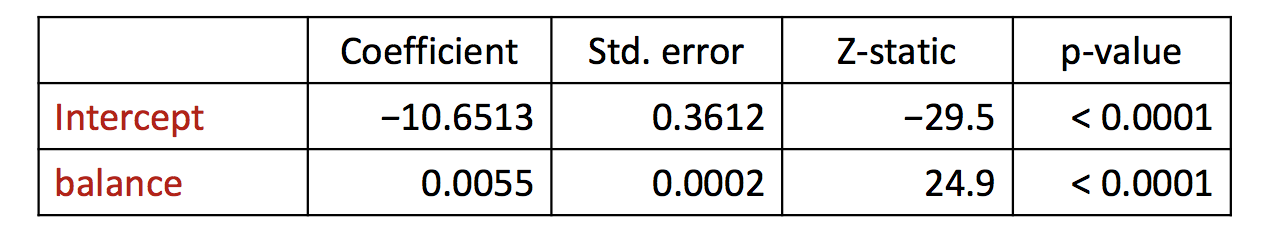
\includegraphics[width=13cm]{img/logit.png}
    \caption{ロジスティック回帰により求められた値}
  \end{center}
\end{figure}
切片($\hat{\beta}_0$)が-10.6513、balanceについて1単位増加させた時の予測変数の増加分$\hat{\beta}_1$が0.0055となるので、例えば$\$ 1000$の人がdefaultする確率は
$$\hat{p}(X) = \frac{\exp{(\hat{\beta}_0 + \hat{\beta}_1 X)}}{1 + \exp{(\hat{\beta}_0 + \hat{\beta}_1 X)}} = \frac{\exp{(-10.6513 + 0.0055 \times 1000)}}{1 + \exp{(-10.6513 + 0.0055 \times 1000)}} = 0.00576$$
よってbalanceが$\$$1000の人がデフォルトする確率は0.5$\%$と極めて低いことがわかる。
質的変数(あるカテゴリに対してそれぞれダミー変数を設定したもの)を用いて予想を行う場合は以下のような学生であるかどうかというダミー変数に対して予測されたパラメータを用いて予測を行う場合、学生である人は$x = 1$、学生でない人は$x = 0$とすれば良いので、学生のデフォルトする確率は
\begin{figure}
  \begin{center}
    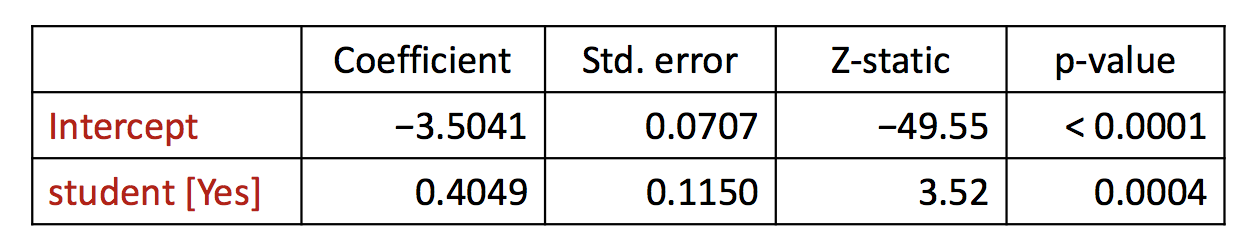
\includegraphics[width=13cm]{img/logit_quali.png}
    \caption{ロジスティック回帰により求められた値(定性情報)}
  \end{center}
\end{figure}
$$\hat{p}(X) = \frac{\exp{(\hat{\beta}_0 + \hat{\beta}_1 X)}}{1 + \exp{(\hat{\beta}_0 + \hat{\beta}_1 X)}} = \frac{\exp{(-3.5041 + 0.4049 \times 1)}}{1 + \exp{(-3.5041 + 0.4049 \times 1)}} = 0.00431$$
上記の式でx=0とした時の確率が0.0292より、学生の方がややデフォルトする確率が高いとこのモデルからは予測できます$\footnote{実際には後述するように必ずしも学生がデフォルトしやすいわけではなく交絡によりそう見えているだけだったりします。}$。
またロジスティック回帰において応答変数(予測するラベル、defaultするかどうか、患者の病気の症状など)が多数の値を取る場合は、ソフトマックス回帰により、最も確率が高くなるラベルを選択肢します。
\begin{itembox}[l]{ソフトマックス回帰}
  ソフトマックス関数は、$n$次元の実数ベクトル $ x = (x_1 \dots  x_n)$を受け取って以下で定義される$n$次元実数ベクトル$y = (y_1 \dots y_n)$を返す関数である。
  $$y_i = \frac{e^{x_i}}{e^{x_1} + e^{x_2} \ldots + e^{x_n}}$$
  ソフトマックス回帰は
  $${\rm softmax}(x)_k = P(Y = k|X) = \frac{e^{x_k}}{\sum_{k=1}^n e^{x_i}}$$
  ここで$e^{x_k} = \exp{(\sum_{p}\beta_{kp}X_p)}$を表し、入力が$X$であるときに予測変数が$k \in K$である確率を表す。
\end{itembox}

\subsection{複数の予測変数を用いたロジスティック回帰}
線形単回帰と同様に、ロジスティック回帰も複数の予測変数を取り入れたモデルに拡張することができます。複数の予測変数を利用したロジスティック回帰を多重ロジスティック回帰といいます。
\begin{itembox}[l]{多重ロジスティック回帰(multiple logistic regression)}
  多数の予測変数を用いたロジスティック回帰モデルを多重ロジスティック回帰という。
  $$ロジット = \frac{p(X)}{1 - p(x)} = \beta_0 + \beta_1 X_1 + \beta_2 X_2 \ldots \beta_p X_p$$
  $$p(X) = \frac{\exp{(\beta_0 + \beta_1 X_1 + \beta_2 X_2 \ldots \beta_p X_p)}}{1 + \exp{(\beta_0 + \beta_1 X_1 + \beta_2 X_2 \ldots \beta_p X_p)}}$$
\end{itembox}

多数ロジスティック回帰についても、計算方法は入力変数を一つにしたロジスティック回帰と基本的には同じです。先ほどと同様に、balance, income, studentを使ってある人がdefaultするかどうかを予測してみます。
\begin{figure}
  \begin{center}
    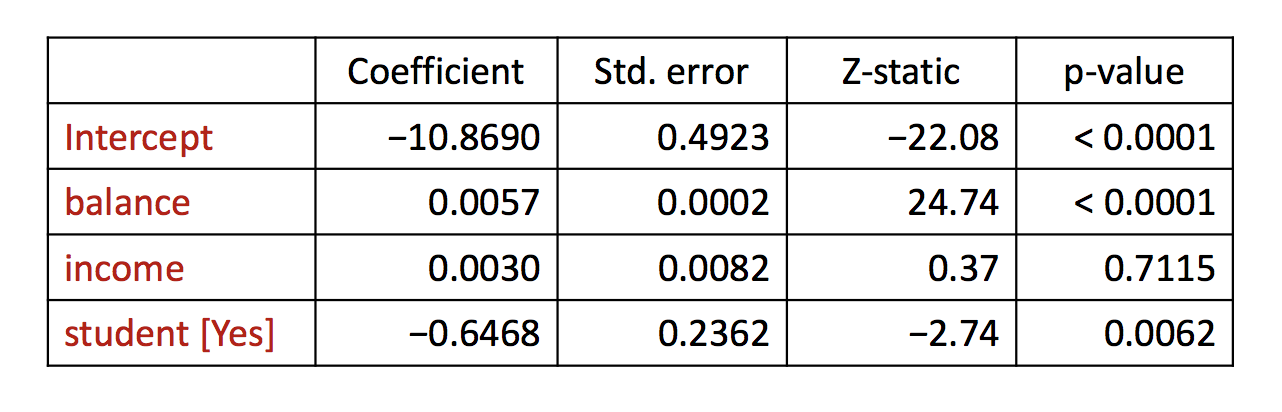
\includegraphics[width=13cm]{img/log_mul.png}
    \caption{多重ロジスティック回帰}
  \end{center}
\end{figure}
balanceが$\$$1,500、incomeが゙$\$$40,000の学生がdefaultする確率は、上の表で切片$ \beta_0 = −10.8690$、balanceにかかるパラメータ$\beta_1 = 0.0057$、incomeにかかるパラメータ$\beta_2 = 0.0030$、studentにかかるパラメータ$\beta_3 = −0.6468$より、\
$$\hat{p}(X) = \frac{\exp{(−10.8690 + 0.0057 \times 1500 + 0.0030 \times 40,000 + (−0.6468) \times 1)}}{\exp{(−10.8690 + 0.0057 \times 1500 + 0.0030 \times 40,000 + (−0.6468) \times 1)}} = 0.058$$
ちなみに式からわかるかもしれませんが、このモデルにおいて学生かどうかを表すダミー変数にかかる$\beta_3 < 0$となっているため、\
同じbalance, incomeであれば\.学\.生\.で\.は\.な\.い方がdefaultする確率は低いと予測されます。これが先ほど軽く補足した交絡(confounding)による効果であり、\
交絡とは統計モデルの中の従属変数と独立変数の両方に(肯定的または否定的に)相関する外部変数が存在することを意味します。例えば「飲酒者と非飲酒者では飲酒者の肺癌発生率が高くなる」というのがデータからは確かに観測されるのですが、\
これは直接的に飲酒が肺がんの要因になっているわけではなく$\footnote{もしかしたら何か関係あるのかもしれないけどそういうのは医学部の人に聞いてください}$、非飲酒者と比較して飲酒者における喫煙者の割合が高いために、\
結果的にデータから「飲酒者の方が肺がんになりやすい」という傾向がでてしまうことになります。今回の問題では実際には学生だからdefaultを起こしやすいのではなく、学生の方が非学と比べincomeが少ない、credit card balanceが大きい等の要因によりデフォルト率が高くなっています。

\subsection{線形判別分析(第7, 8講)}
ロジスティック回帰のように直接${\rm Pr}(Y| X = x)$ をモデル化するのではなくある入力変数$X$が与えられた時にそれがある応答変数$Y$となる確率を予測する別のモデルに「線形判別分析(LDA)」があります。\
\begin{itembox}[l]{線形判別分析(linear discriminant analysis)}
  線形判別分析とは、${\rm Pr}(Y| X = x)$を正規分布でモデル化し、ベイズの定理によって${\rm Pr}(Y| X = x)$を計算するモデル。
  $K$をクラスの数、$\pi_k$をラス$k$の事前分布、$f_k(x)$をクラス$k$のデータの密度関数とすると、${\rm Pr}(Y| X = x)$は以下のように表される。
  \begin{equation}
    \begin{split}
      {\rm Pr}(Y| X = x) &= \frac{{\rm Pr}(Y = k){\rm Pr}(X = x| Y = k)}{{\rm Pr}(X = x)} \\
      &\frac{{\rm Pr}(Y = k){\rm Pr}(X = x| Y = k)}{\sum_{l=1}^K{\rm Pr}(X = x, Y = l)}\\
      &=\frac{{\rm Pr}(Y = k){\rm Pr}(X = x| Y = k)}{\sum_{l=1}^K{\rm Pr}(Y = l){\rm Pr}(X = x|Y = l)}\\
    \end{split}
  \end{equation}
    \begin{equation}
      p_k(x) = \frac{\pi_kf_k(x)}{\sum_{l=1}^K \pi_lf_l(x)}
    \end{equation}
\end{itembox}
$f_k(x)$が正規分布だと仮定すると、$f_k(x)$は以下の式で表される。
\begin{equation}
  f_k(x) = \frac{1}{\sqrt{2\pi}\sigma_k}\exp{\left(- \frac{1}{2\sigma_k^2}(x - \mu_{x_k})^2\right)}
\end{equation}
分散が全てのクラスで等しい場合、ある入力$x$が与えられた時、それが$k$である確率は式(5)を式(4)に代入することで求めることができ、\
\begin{equation}
        p_k(x) = \frac{\pi_k \frac{1}{\sqrt{2\pi}\sigma_k}\exp{\left(- \frac{1}{2\sigma_k^2}(x - \mu_{x_k})^2\right)}}{\sum_{l=1}^K \pi_l\frac{1}{\sqrt{2\pi}\sigma_l}\exp{\left(- \frac{1}{2\sigma_l^2}(x - \mu_{x_l})^2\right)}}
\end{equation}
式(6)より、$p_k(x)$は$\pi_k \frac{1}{\sqrt{2\pi}\sigma_k}\exp{\left(- \frac{1}{2\sigma_k^2}(x - \mu_{x_k})^2\right)}$に比例するため、\
これが最も大きくなるクラスに入力データを分類すればいいことがわかります。
これについて対数をとると
$$\log{\pi_k} + \log{1} - \log{\sqrt{2\pi}\sigma} + \left(-\frac{1}{2\sigma^2}(s - \mu_k)^2 \right)$$
となり、予測に関わるのは$\pi_k$を含んだ項のみとなるため、

$$\log{\pi_k} + x \frac{\mu_k}{\sigma^2} - \frac{\mu_k^2}{2\sigma^2} = \delta_k(x)$$

として、この$\delta_k(x)$を最大にするクラス$k$に事例$x$を分類すると考えることができます。
すなわちK個のクラスに対して$\mu_k及び\sigma_k^2$がわかれば分離境界$x$を求めることができます。\\
例えば$K=2, \pi_1=\pi_2, 等分散性より\sigma_1 = \sigma_2 = \sigma$の場合を考えると、分離境界において$\sigma_1(x) = \sigma_2(x)$が成立するため、
$$x\frac{\pi_1}{\sigma^2} - \frac{\mu_1^2}{2\sigma^2} + \log{\pi_1} = x\frac{\pi_1}{\sigma^2} - \frac{\mu_2^2}{2\sigma^2} + \log{\pi_2}$$
$$x = \frac{\mu_1 + \mu_2}{2}$$
実際には$\mu_k及び\sigma_k^2$は未知なので、以下のようにデータから推定し判別関数を求めます。
\begin{itembox}[l]{$\hat{\mu}_k及び\hat{\sigma}_k^2$の推定による線形判別分析法による分類}
  $n$を学習データの全事例、$n_k$を クラス$k$に属する事例の数とすると、
  $$\hat{\mu}_k = \frac{1}{n_k}\sum_{i:y_i =k}^k x_i,\ \hat{\sigma}_k^2 = \frac{1}{n−K}\sum_{k=1}^K\sum_{i:y_i=k}(x_i - \hat{\mu}_k)^2$$
  また$\pi_k$も未知である場合は以下のようにデータから推定できる。
  $$\hat{pi}_k = \frac{n_k}{n}$$
  線形判別分析ではこれらの推定値を用いて、以下の判別関数$\hat{\sigma}_k$が最も大きくなるクラスに分類する。
  $$\hat{\sigma}_k = x\frac{\hat{\mu_k}}{\hat{\sigma}_k^2} - \frac{\hat{\mu_k}^2}{2\hat{\sigma}_k^2} + \log(\hat{\pi}_k)$$
\end{itembox}
予測変数が2以上の場合は密度関数が異なるので判別関数が異なるのですが基本的な求め方が前述の方法と同じなのと、あの式を入力するのがめんどくさいのでスライドで確認していただけると嬉しいです。

\subsection{二次判別分析}
線形判別分析では各グループは多変量正規分布をしており、かつ等分散性(全てのグループが同じ共分散行列を持つ)を持つことを仮定していました。二次判別分析ではクラスごとに異なる共分散行列を想定し、判別を行います。\
\begin{itembox}[l]{二次判別分析(quadratic discriminant analysis, QDA)}
  クラスごとに異なる共分散行列を想定し、以下の判別関数の与えるスコアが最も大きくなるクラス$k$に分類する。
  % $$X \~ N(\mu_k, \)$$
  $$\delta_k(x) = -\frac{1}{2}x^T\sum_k^{-1}x + x^t\sum_k^{-1}\mu_k - \frac{1}{2}\mu_k^T\sum_k^{-1}\mu_k - \frac{1}{2}\log{|\sum_k|} + \log{\pi_k}$$
\end{itembox}
QDAではクラスごとに分散共分散行列のパラメータを求める必要があり、計算のコストが大きくなることまた学習パラメータが小さいときなどは学中データにフィットしすぎて過学習を引き起こす可能性があります。(バリアンスが大きく、バイアスが小さい)\
一方LDAはバリアンスは小さいものの、そもそも共分散行列が各クラスで同じという過程をおいているため、そもそもこの過程が成立していなかった場合、データにフィットせずバイアスが大きくなる恐れがあります。

\subsection{分類手法の比較}
では分類問題においてはこれまで取り扱った「ロジスティック回帰」「線形判別分析」「虹判別分析」「K最近傍法」のうち、どの判別器を用いるのが良いのでしょうか。
まずロジスティック回帰及びLDAでは共に境界面が直線(もしくは超平面)になるため、そもそも線形分離のできないデータには十分に対応できません。仮にデータが線形分離が可能な場合はデータの分布が各クラスそれぞれ正規分布である時は、これを仮定においてモデルを構築するLDAの方がやや精度が高くなります。\
KNN、QDAは共に非線形な決定境界を実現可能ですが、KNNはより複雑な境界線を構築することができる一方、前述の通り多くのデータを必要としかつ結果からどのパラメータが重要なのか等がわかりにくいため、学習データが少ない時はQDAの方が良いというべきかもしれません。
\begin{itembox}[l]{分類手法の比較についてのまとめ}
  \begin{description}
    \item [LDA]\mbox{}\\
    真の決定境界が線形かつデータの分布が各クラスそれぞれ正規分布に従っている。また分散共分散行列が等しい。
    \item [ロジスティック回帰]\mbox{}\\
    真の決定境界が線形かつデータの分布が各クラスそれぞれ正規分布に従っていない。
    \item [QDA]\mbox{}\\
    真の決定境界が非線形かつデータの分布が各クラスそれぞれ正規分布に従っている。分散共分散行列が等しくない。
    \item [KNN]\mbox{}\\
    決定境界の非線形性か特に゙強い場合もしくは非線形性があり、データが正規分布に従っていない時。
  \end{description}

\end{itembox}

\subsection{正解率以外の評価指標}
分類問題においては、単なる正解率(accuracy)以外にもいくつか評価指標があり、クラスによりデータの数が大きく異なる時$\footnote{例えば婚活アプリのチャットのログからどういったやりとりをしている二人が実際に付き合っているのかを予測したい時、全体の中で実際にカップル成立したログのデータが10$\%$以下しかなかったとすると、\
「全ての組み合わせが結局付き合うに至らなかった」と予測するようなでたらめなモデルでも正解率を見ると9割以上になってしまいます。しかしここで知りたいのはデータの中で少数派の「どういったやりとりをした二人が実際に付き合ったのか」であり、\
この少数派をきちんと予測できるモデルを評価できる指標を用いる必要があります。}$問題によってはこれらの評価指標がモデルの評価基準として適していることがあります。授業で紹介されていたのはsensitivityとspecificity及びROC曲線でありこれらの評価指標は主に二値分類で用いられます。\
\subsubsection{感度(sensitivity)と特異度(specificity)}
それぞれ、実際のラベルがYesであるもの、Noであるものに対して正しく予測ができているのかを測る指標です。\
図8のようにデータを実際のラベルと予測結果で分割したものを混同行列(confusion matrix)といいます。
\begin{figure}
  \begin{center}
    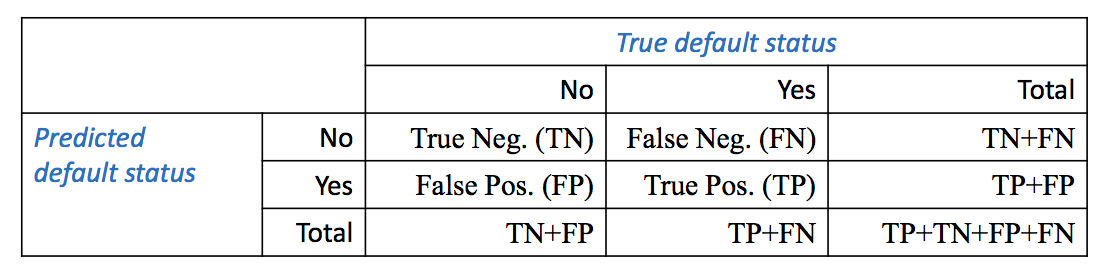
\includegraphics[width=13cm]{img/sens.png}
    \caption{混同行列}
  \end{center}
\end{figure}
\begin{itembox}[l]{sensitivityとspecificity}
  \begin{description}
    \item [感度(sensitivity)]\mbox{}\\
    実際のラベルが「Yes」であるものに対してきちんとモデルが「Yes」と予測できているかどうか。(Yesであるものを正しく検出できた割合)
    $${\rm sensitivity = \frac{TP}{TP + FN}}$$
    \item [特異度(specificity)]\mbox{}\\
    実際のラベルが「No」であるものに対してきちんとモデルが「No」と予測できているかどうか。(Noであるものを正しく検出できた割合)
    $${\rm sensitivity = \frac{TN}{TN + FP}}$$
  \end{description}
\end{itembox}
混同行列のそれぞれのブロックに対応したカテゴリ名がややわかりにくいかもしれませんが、「予測結果=実際の分類」であればTrueが頭につき、「予測結果がYes」であればPositiveが次に、「予測結果がNo」であればNegativeが後につきます。\
つまり「本来のラベルはNoだがYesだと予測されてしまった」ケースについては、実際のラベルと予測が異なるので頭に「False」が予測結果がYesなので後ろにPositiveがつき「False Positive(偽陰性)」になります$\footnote{個人的に忘れにくい覚え方は「結婚相手を探す時にFalse Positive」だけは引っかかってはいけない」\
(本来ならうまくいくはずのない相手と誤って結婚してしまい、そういう結果になること)です。}$。
実際に感度、特異度を求めたい場合はここにそれぞれの値を代入するだけでいいです。
特に「Yes」が全体の中で閉める割合の低いデータについてはモデルにより「Yes」が想起される確率が低くなります。\
これをそのまま放置すると「全てをNoで分類するモデル」になりかねないので、あえて閾値0.5ではなく0.2等に下げることで本来の二値分類では「No」に分類されていた事例も「Yes」に分類されやすくなり感度を高くすることができます。\
ただこの場合当然ですがエラー率は上がってしまうため、目的に応じてこういった指標を使い分ける必要があります。
sensitivity、specificity以外に図9のようにもいくつか指標はありますが、授業で詳しくは触れていないので特に大丈夫だと思います。
% \begin{figure}
%   \begin{center}
%     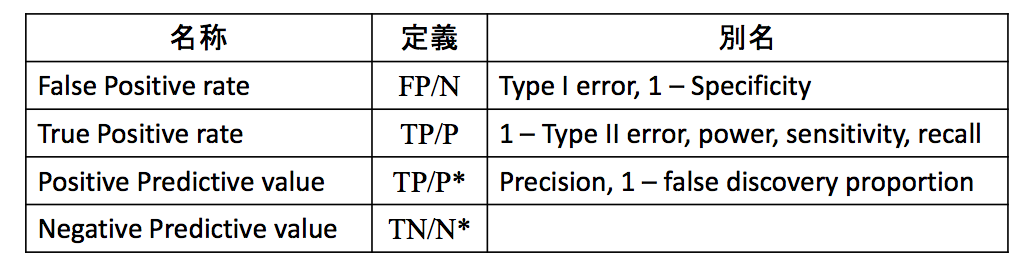
\includegraphics[width=13cm]{img/sihyo.png}
%     \caption{混同行列}
%   \end{center}
% \end{figure}
\begin{figure}[htbp]
\begin{minipage}{0.5\hsize}
 \begin{center}
  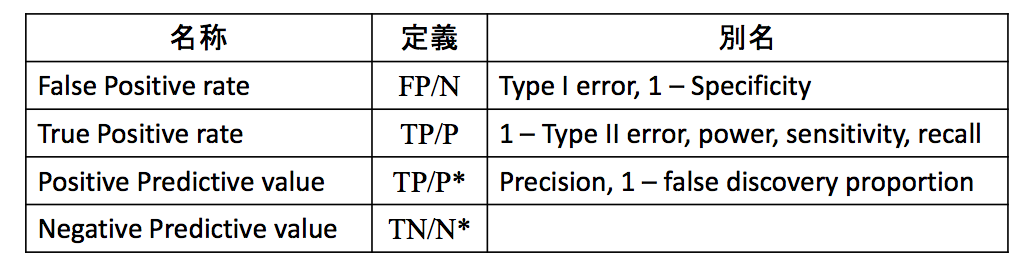
\includegraphics[width=70mm]{img/sihyo.png}
 \end{center}
 \caption{様々な評価指標}
 \label{fig:one}
\end{minipage}
\begin{minipage}{0.5\hsize}
 \begin{center}
  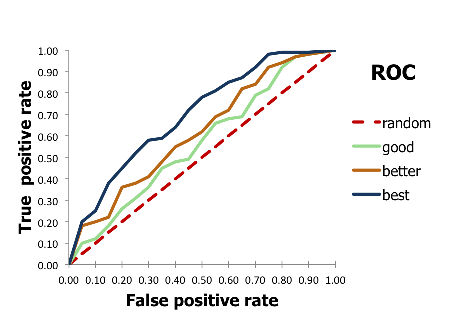
\includegraphics[width=70mm]{img/ROC.png}
 \end{center}
 \caption{ROC曲線}
 \label{fig:two}
\end{minipage}
\end{figure}
\subsubsection{ROC曲線(receiveroperatingcharacteristicscurve)}
上のように特にデータの中で偏りがある場合などに閾値をあえて0.5ではなくそれ以下もしくは以上にすることにより目的とする結果をえられるモデルを作りたい時があります。\
これも交差検証で適切な閾値の結果を探す必要があるのですが、その場合はこれまでのように正解率ではなくAUC(Area Under the Curve)という指標を用います。\
まず、False Positive Rate(= 1 - Specificity)とTrue Positive Rate(= Sensitivity)をそれぞれ$xy$平面にプロットします。この結果えられた曲線をROC曲線といい、\
このROC曲線の下の部分の面積をAUCといいます。このAUC値が1に近いほど判別能が高いことを示しています。図10からもわかるようにROC曲線の下の面積が大きいものほど優れたモデルになります。
% \begin{figure}
%   \begin{center}
%     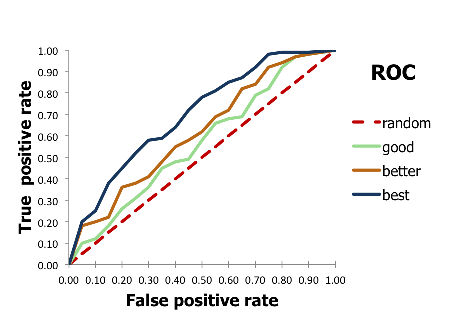
\includegraphics[width=13cm]{img/ROC.png}
%     \caption{混同行列}
%   \end{center}
% \end{figure}
閾値を変えて予測を行った際にAUCが最もよくなる閾値を選択します。

\section{リサンプリング法(第9講)}
リサンプリング法とは、手持ちの限られたデータをある固定された割合で分割し、訓練データとテストデータに分けて学習するのではなく、\
ランダムサンプリングと学習によるパラメータ推定を複数回行い、データの分割の仕方による予測モデルのばらつきなどを少なくすることを目指しています。\
試行回数が増える分計算コスト画像化するため、かつてはこれがネックになっていましたが、計算機の能力向上によりこういったコストの問題は小さくなっています。\
以下で代表的なリサンプリング手法について紹介します。
\subsection{検証セットによる手法}
データセットをランダムに「学習用データセット(training set)」と「検証用データセット(validation set)」の二つにランダムに分割し、\
学習用データでモデルのパラメータを推定し、検証用データで精度を評価するという、最もベーシックな方法です。シンプルな一方で、\
データをどう分割するかによって精度の推定値やパラメータの予測値は大きく変わってしまうこと、\
またデータ自体が少ない時にデータ全体の数割から半分ほどのデータを学習に用いることができないため、精度も本来達成可能な精度より低めに推定される可能性があります。

\subsection{交差検証}
検証セットによる精度測定法を補うため、交差検証法はデータセットの全てのデータを用い、また繰り返し学習したパラメータの平均値を取ることでデータの分割の仕方によるばらつきの影響を排除することを目指しています。
\begin{itembox}[l]{Leave-One-Out Cross Valdation(LOO交差検証)}
  $N$個の学習データ${(x_1, y_1),\ (x_2, y_2) \ldots\ (x_n, y_n)}$のうち、1つをのぞいた$N-1$個で学習を行い、毎回残された1個のデータで性能を評価、\
  これを全ての事例に対して行いその$MSE$の平均をとることで、最終的な評価指標の推定値とする。\\
  $$ {\rm MSE_1} = (\hat{y}_1-y_1)^2$$
  $$\dots$$
  $$ {\rm MSE_n} = (\hat{y}_n-y_n)^2$$
  $$ {\rm CV(n)} = \frac{1}{n}\sum_{i=1}^n MSE_i$$
\end{itembox}
LOO交差検証には以下のようなメリットデメリットが存在します。
  \begin{description}
    \item [LOO交差検証のメリット]\mbox{}\\
    学習には毎回n-1個のデータが使用されn個全てのデータを用いた際とほぼ同じ性能のモデルを作ることができる。\
    また分割方法の違いによる性能評価のばらつきもない。
    \item [LOO交差検証のデメリット]\mbox{}\\
    n回の学習が必要になり、かつ学習データと検証データに一定割合で分割する際と比べ学習に\
    使用するデータの数も増えるため、データの数が多いほど、学習に必要なコストが大きく増加する。
  \end{description}

このように、LOO交差検証は学習データと検証データに分割する際のデメリットを克服できる一方、\
計算コストが大きく増加してしまいます。そこで、一つだけを性能評価用に残し、$n$回学習を行うのではなく、\
データをある数$k$に分割し、一つのグループ以外のデータで学習、残された一つのデータで性能検証を行うことを繰り返すことで\
計算量を抑えつつも性能の向上を目指すのが次のk分割交差検証です。
\begin{itembox}[l]{k-fold Cross Valdation(k分割交差検証)}
  データを$k$個のグループに分割し一つを検証データ、残りの$k+1$個を学習データとしてMSEを計算し、これをk回繰り返して平均を取り、\
  この平均をテストMSEとして推定する。一般的に$k=5, 10$等が用いられる。
  $$CV(k) = \frac{1}{k}\sum_{i=1}^k {\rm MSE}_i$$
\end{itembox}
LOO交差検証では一般にn回の学習を行う必要があったが、$k$分割時交差検証では学習回数はたかだか$k$回ですむ一方、LOO交差検証と同様、\
$k$回の学習を通して全ての入力データをみることができます。またLOO及び$k$分割交差検証の間には以下のようなBias-variance trade-offが存在します。
% \begin{itembox}[l]{Bias-variance trade-off}
  \begin{itemize}
    \item $k$分割交差検証の場合、学習に使えるデータの数はLOO比べ少なくなるので、バイアスが大きくなる可能性がある。
    \item LOO交差検証には学習に使うデータが毎回ほとんど同じなので出力間に強い相関があり、バイアスが大きい。
  \end{itemize}

% \end{itembox}
\subsection{ブートストラップ}
また、こういったデータを分割し、繰り返し学習左折以外に、ブートストラップという方法もあります。
 \begin{itembox}[l]{ブートストラップ}
   標本からの復元抽出によるランダムサンプリングを繰り返すことで行う統計的推論手法。確率モデルのパラメータの信頼区間などを簡単に求めることができる。
 \end{itembox}
 復元抽出とは、抽出を行う際に一度抽出したサンプルが再び抽出の対象となりうる方法のことです。例えば受験数学でよくでてくる「赤い玉3個、白い玉4個入った袋から中身を見ずに一個取り出し色を確認して戻す作業を3回行った時、\
 全て赤い玉であった確率は」などは復元抽出の例であり、「一度出した玉は元に戻さない」であればこれは非復元抽出になります。具体的なブートストラップ法の利用としては、
 \begin{enumerate}
   \item 手持ちのデータセットからランダムサンプリングによって新たなデータセットを生成。
   \item この抽出されたデータを元にモデルのパラメータを推定する。
   \item これを多数回繰り返す。
   \item 得られたパラメータの分布より信頼区間などを計算する。
 \end{enumerate}
という手順になります。

\section{正則化(第10講)}
\subsection{パラメータ推定法と縮小推定法}
最小二乗法、最尤推定法などのパラメータ推定法では、モデルがデータにフィットするようにパラメータを最適化します。\
一方リッジ回帰、Lasso回帰は縮小推定に分類され、各パラメータの絶対値が大きくならないようにする。正則化ともいう。\
最小二乗法による線形回帰パラメータ推定は、以下の{\rm RSS}を最小化にするパラメーラ$\beta_0, \beta_1..., \beta_p$を決定します。\
これは学習データへのフィティングしか考慮していないため、過学習してしまいやすく、未知のデータに対して適切に予測できない恐れがあります。\
そこでリッジ回帰やLasso回帰などの縮小推定法により過学習を回避し、未知データに対しても頑健なモデルを構築します。

\subsection{リッジ回帰}
\begin{itembox}[l]{リッジ回帰}
  リッジ回帰の目的関数は以下で表される。
  $$\sum_{i=1}^n \left(y_i - \beta_0 - \sum_{j=1}^p \beta_jx_{ij}\right)^2 + \underline{\lambda \sum_{j=1}^p \beta_j^2}$$
下線で示され項がパラメータの絶対値が大きくなることに対するペナルティ(L2正則化項)となる。\\
$\lambda$ : チューニングパラメータ。
\end{itembox}
L2正則化項の$\lambda$を大きくするほど、各パラメータの値$\beta_0, \beta_1..., \beta_p$はゼロに近づいていくことになります。\
またリッジ回帰においては、値の大きな予測変数が大きな影響力を持つようになるため、予測変数のスケールが性能に大きな影響を与えてしまいます。\
そのため前処理として以下のような式で予測変数の標準化を行う必要があります。
\begin{equation}
  \widetilde{x_{ij}} = \frac{x_ij}{\sqrt{\frac{1}{n} \sum_{i=1}^n (x_ij - \overline{x_j})^2}}
\end{equation}

$\lambda$を大きくするとバリアンスは小さくなり、バイアスは大きくなります。これは$\lambda$が小さければ、リッジ回帰の目的関数はパラメータ推定法における目的関数と近く、つまり学習データへの\
過学習によりバリアンス(入力データによる出力結果のばらつき)が大きくなる傾向にある一方、$\lambda$が大きければモデルは過学習を抑え新しい学習データに対しても頑健になるためバリアンスは小さるためです。\
その一方で、$\lambda$項を大きくすると元の学習データに対するフィットは少なくなるためバイアスが大きくなります。
ここでも以下の式で表されるバイアスバリアンスのトレードオフ関係が存在します。
\begin{equation}
  E[(y_0 - \hat{f}(x_0))^2] = {\rm Var}(\hat{f}(x_0)) + [{\rm Bias}\hat{f}(x_0)]^2 + {\rm Var}(\epsilon)
\end{equation}
バイアス、バリアンスが共に大きくなりすぎず、MSEが最小になるちょうどいい$\lambda$を交差検証等を行って選択することにが大事です。
% \begin{figure}
%   \begin{center}
%     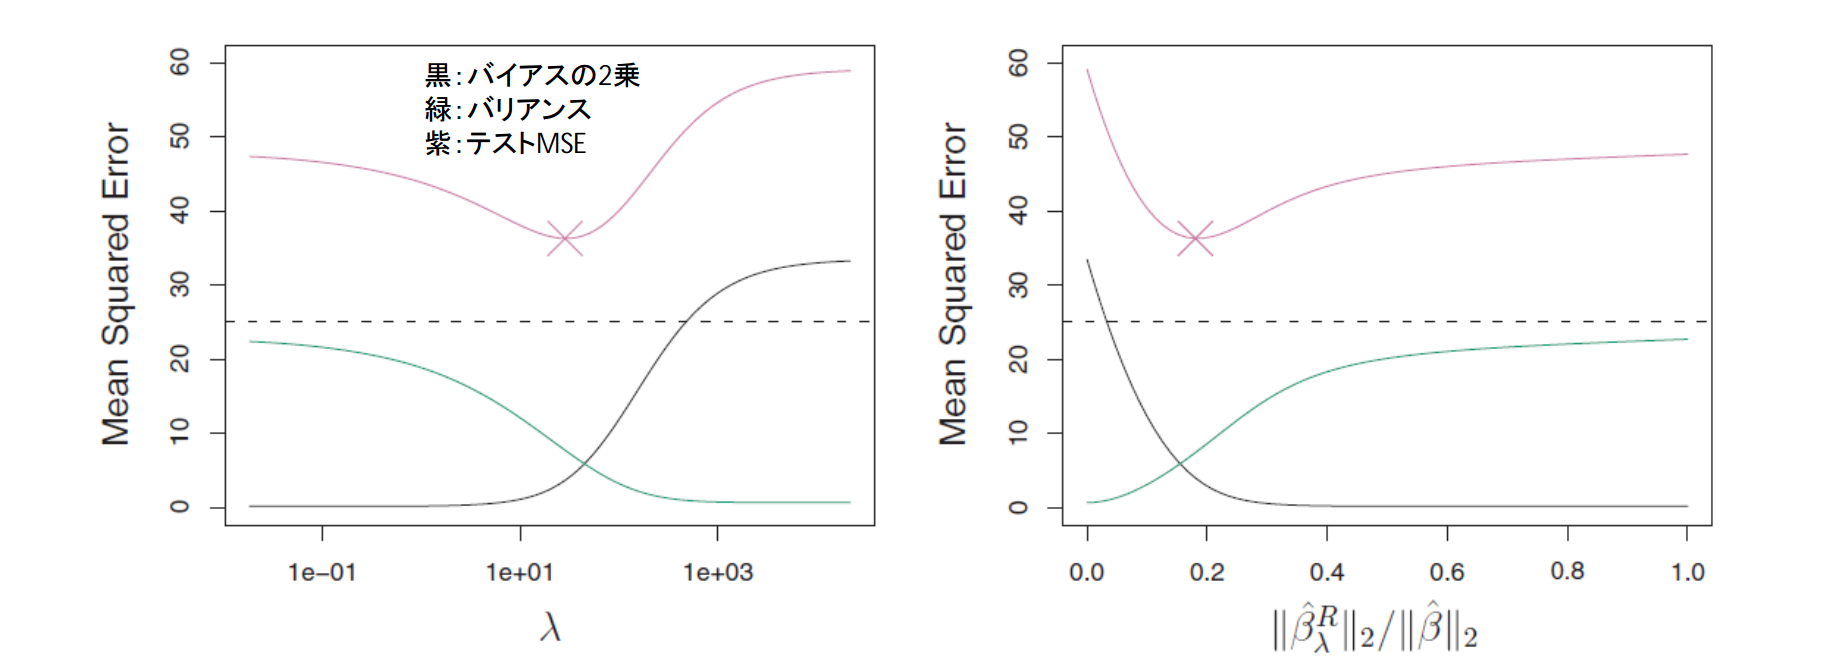
\includegraphics[width=13cm]{img/lidge_lambda.png}
%     \caption{Creditデータセットに対してリッジ回帰}
%   \end{center}
% \end{figure}
%以下のグラフのバツ印のところで、バイアス、バリアンス共に小さくなっており、予測において使用すると良い$\lambda$の値になっていることがわかります。

\subsection{Lasso回帰}
Lasso回帰は、正則化項をパラメータの二乗ではなく、絶対値とした目的関数を最小化することによりパラメータを求める方法です。
\begin{itembox}[l]{Lasso回帰}
  Lasso回帰の目的関数は以下で表される。
  $$\sum_{i=1}^n \left(y_i - \beta_0 - \sum_{j=1}^p \beta_jx_{ij}\right)^2 + \underline{\lambda \sum_{j=1}^p |\beta_j|}$$
下線で示され項がパラメータの絶対値が大きくなることに対するペナルティ(L1正則化項)となる。\\
$\lambda$ : チューニングパラメータ。
\end{itembox}

Lasso回帰の目的関数はリッジ回帰と比べ、最後の正則化項が異なっているだけに見えますが、この式から得られるパラメータの性質は大きく異なります。\
リッジ回帰ではパラメータ$\beta$が0に近づくにつれ、L2正則化項はそれぞれのパラメータを二乗したものの総和なので、より急速に0に近づきます。一方Lasso回帰では、正則化項は$beta$の絶対値の和になるため、\
L1正則化項は$\beta$に比例して小さくなり残り続けます。結果としてLasso回帰では$\lambda$の値を大きくするにつれ、多くのパラメータが急速に0に近づくため、より重要なパラメータ以外の\
枝葉のパラメータが自動的に除かれることになります。特に多くのパラメータを保持したくない場合(例えば携帯端末に保存するモデルを作るときなど)はこちらの方が適していると言えます。\
図8はCreditデータセットに対してLasso回帰を行い、$\lambda$を大きくした際のパラメータと出力のCoefficientを示しており、$ \lambda$が大きく\
なるにつれて、多くのパラメータが急速に0に近づいていることがわかります。(ここら辺は授業でやった手計算で自分で確認してみるとわかりやすいと思います。余裕があれば参考資料で補足します。)
\begin{figure}
  \begin{center}
    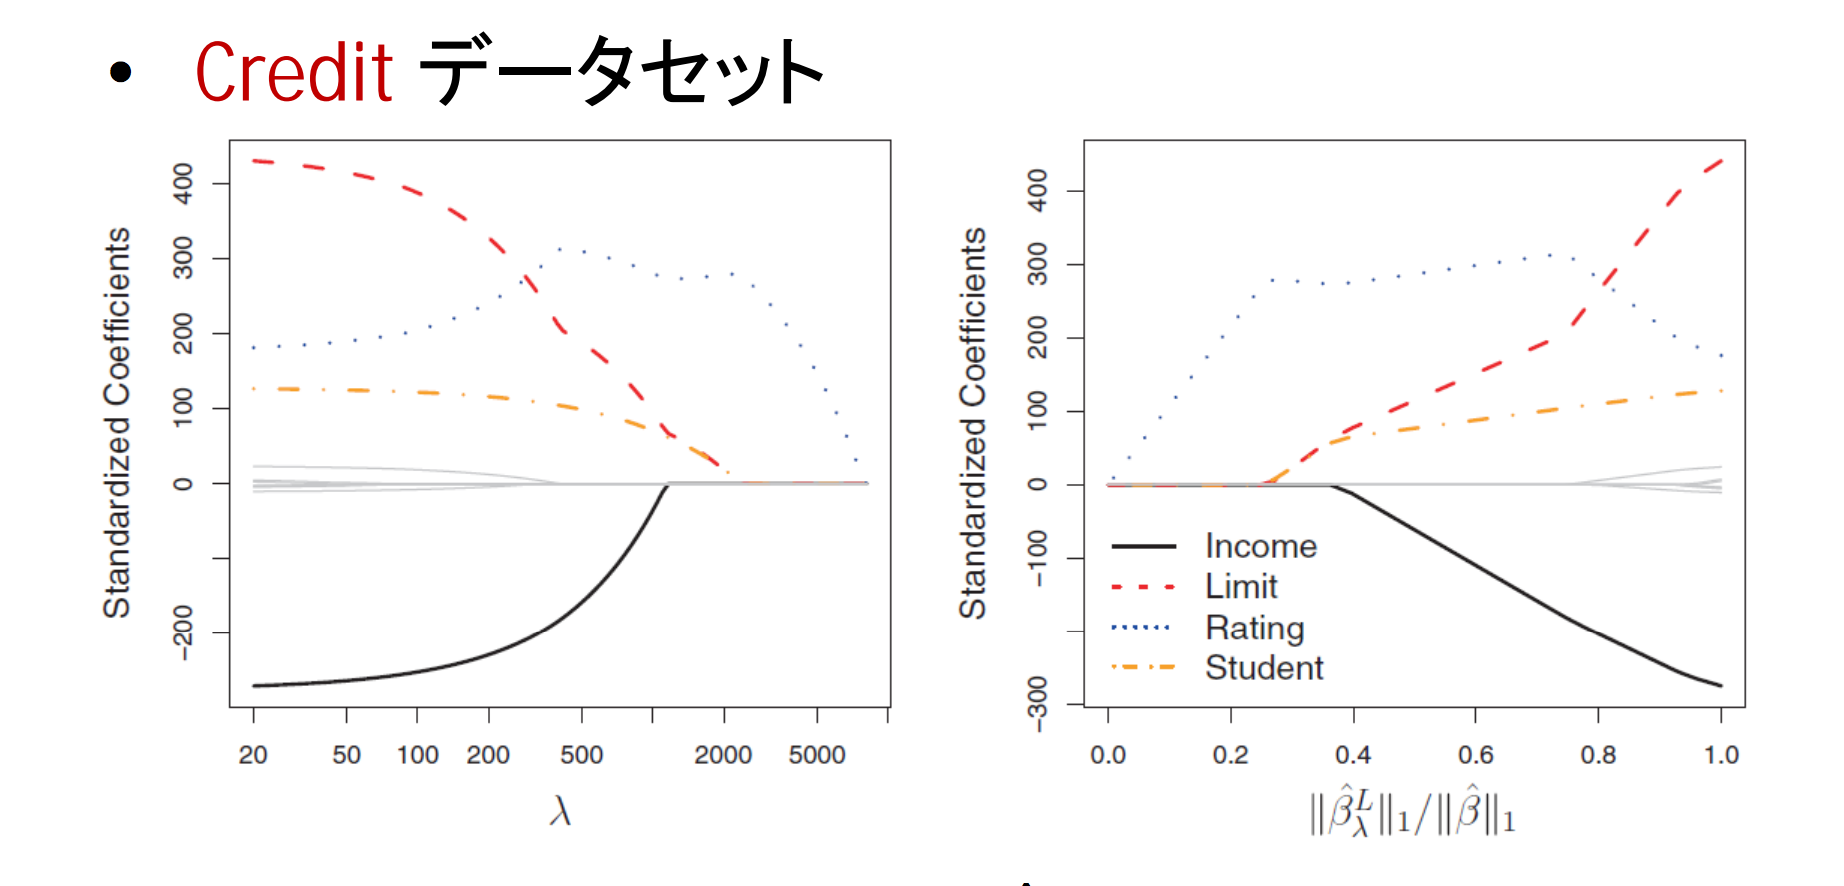
\includegraphics[width=13cm]{img/lasso_lmd.png}
    \caption{Creditデータセットに対してLasso回帰}
  \end{center}
\end{figure}

リッジ回帰、Lasso回帰どちらが適切なのかはデータの性質によって異なり、また、適切な$\lambda$の選択については、交差検証によってもっともTest MSEが小さくなる$\lambda$を選択する必要があります。\
最適化(パラメータ推定)の際には絶対値項を持っているためにL1正則化の方が勾配の計算が難しくなる。L2は二乗の総和でしかないのでが並んでいるだけなので勾配計算が簡単であり、Lasson回帰の方が最適化が難しくなってしまうという短所があり、\
特にデータサイズが大きい時は勾配の計算(数値計算)が面倒になります。

%beta_iで変二分するとiの部分だけ残る
%らら
% \subsection{交差検証による$\lambda$のチューニング}
% リッジ回帰、Lasso回帰における正則化項にかかる係数$\lambda$の調整においては以前の項で紹介された交差検証により行います。様々な $\lambda$の値に対して交差検証でTest MSE を推定し、最も精度が良くなる$\lambda$を選びます。\
% ゙そのほか補足
% Elastic Net->L1正則化項とL2正則化項の両方を追加 \\

\subsection{高次元データでの学習(第11講)}
入力データによっては、予測変数(特徴量)$p$が学習事例の個数$n$よりも大きくなることが大きくなることがあります。例えば、血圧の予測では、特徴量として年齢、性別、BMIの他に遺伝子情報(SNPs)を特徴量として入れる場合、
遺伝子情報は個々人によって少しずつ異なり、それぞれにダミー変数を振り分けていくと予測変数の数は膨大に増加する($p \approx 500000$)。仮に患者データが200人分ほど($n \approx 200$)であれば$p \gg n$となってしまいます。\
他にもスパムメールの分類で単語を特徴量として用いる時、すでに{スパム、スパムでない}のラベルがついたメールが1000件前後しかない時に、そこに含まれている全ての単語を特徴量として用いれば$\footnote{単語を特徴量として用いる場合は基本的にはある文章にある単語が含まれているかどうかに基づいて特徴量をつけます。\
ただここで他の質的変数のように0/1の二値で値をつけると、文章の中である単語が他と比較して多く出現しているなどの情報を生かしきれなくなります。実際にはtf-idfという手法を用いて文章を$n$種類の単語に対応したベクトルに変換することが2000年代までは主流でした。ちなみに深層学習モデルにおいては単語の離散表現(それぞれの単語を\
数百次元のベクトルで表現する)を用いることが一般的です。}$、\
特徴量の数はデータの数をたやすく上回ってしまいます。$p \geq n$のとき、必要ではないノイズな予測変数(例えばスパムメール内でも実際には分類に大きく関係しない単語は多々存在しています)でもフィットしてしまうため、\
過学習に陥る可能性が高くなります。

これに対する対処法としては、正則化や変数選択などによりモデルの柔軟性を下げ、必要ではない予測変数を減らします。しかしこの方法にはいくつか注意点があり、例えば多重共線性$\footnote{ある変数間で相関がある時、それが解析に支障が出るほどX同士の相関が強い時に、「多重共線性(たじゅうきょうせんせい)があると言います。\
http://xica.net/vno4ul5p/}$により、変数選択によって選ばれた変数以外にも有用な変数が存在する可能性があります。\
また学習データで得られる{\rm RSS}や決定係数は、実際のデータでも完全に当てはまるとはいえず、モデル の性能の指標としては無意味であることも注意が必要です。

\section{決定木(decision tree)}
木構造によって回帰や分類のための条件を表すモデルであり、目的とする問題に応じて回帰木(regression tree)、分類木(classification tree)があります。\
\subsection{回帰木}
回帰木とは、ある数値(連続値)の推定のルールをツリーで表現したものです。
Hittersデータセット$\footnote{https://vincentarelbundock.github.io/Rdatasets/doc/vcd/Hitters.html}$は、選手の在籍年数(Years)と打数(Hits)よりLog(Salary)を予測するデータセットです。回帰木を用いてSalaryを予測する時、図9のようにまず「Years $<$ 4.5」なら選手のLog(Salary)は5.11に決定され、\
そうでない、かつ「Hits $<$ 117.5」ならば6.00、「Years $<$ 4.5」かつ「Hits $\geq$ 117.5」ならば6.74となる。
% \begin{figure}
%   \begin{center}
%     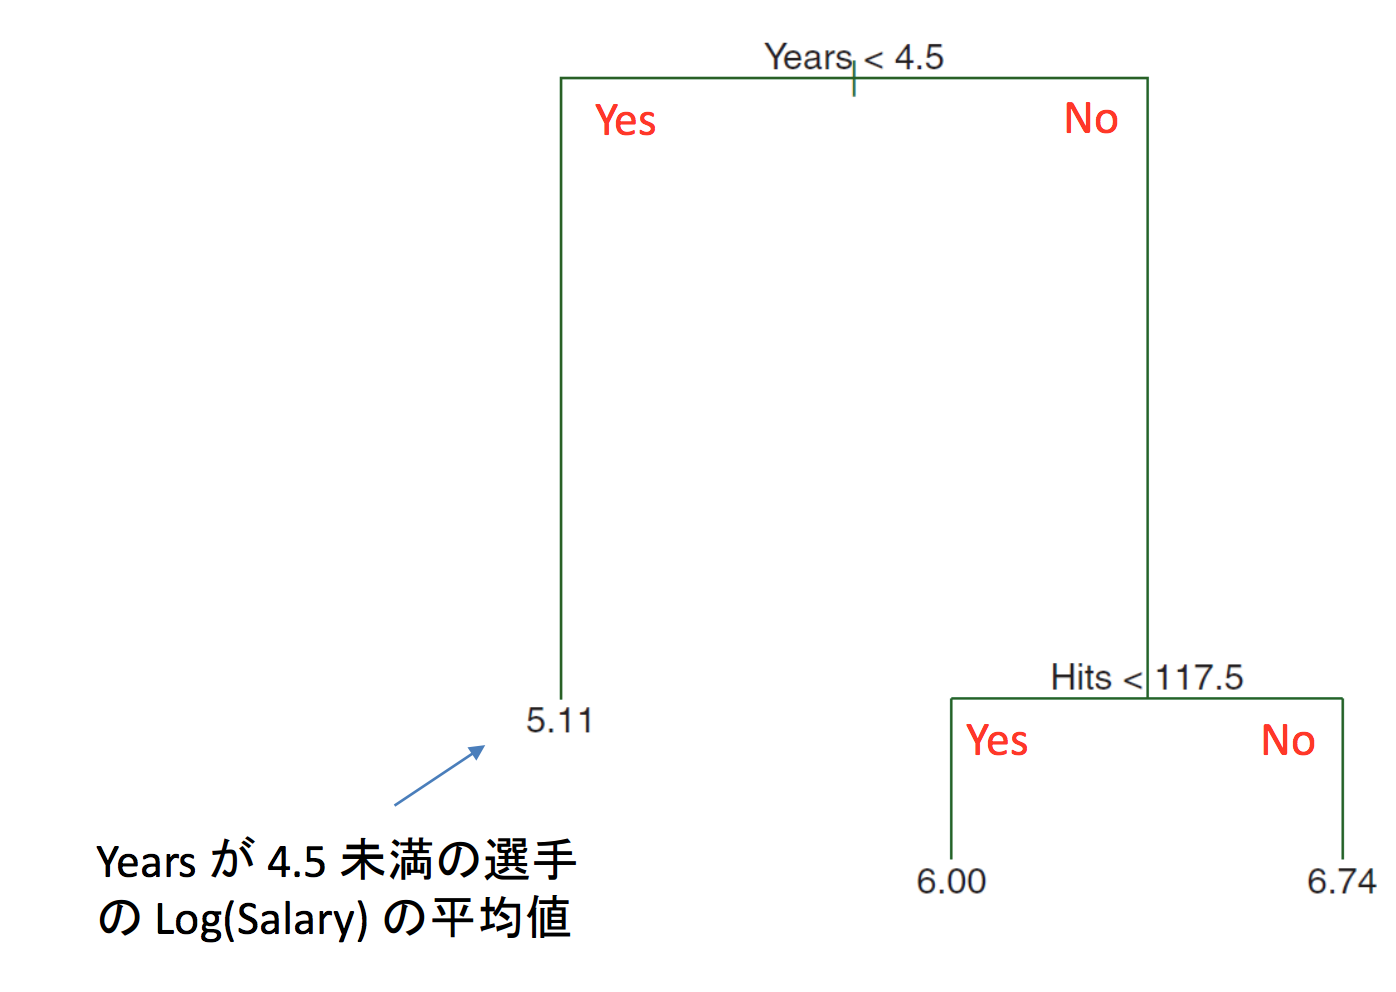
\includegraphics[width=10cm]{img/kaikiki.png}
%     \caption{Hittersデータに対する回帰木予測}
%   \end{center}
% \end{figure}

回帰木は予測変数の空間を$K$個のリージョンに分割することにより、分岐条件を求めます。
\begin{figure}[htbp]
\begin{minipage}{0.5\hsize}
 \begin{center}
  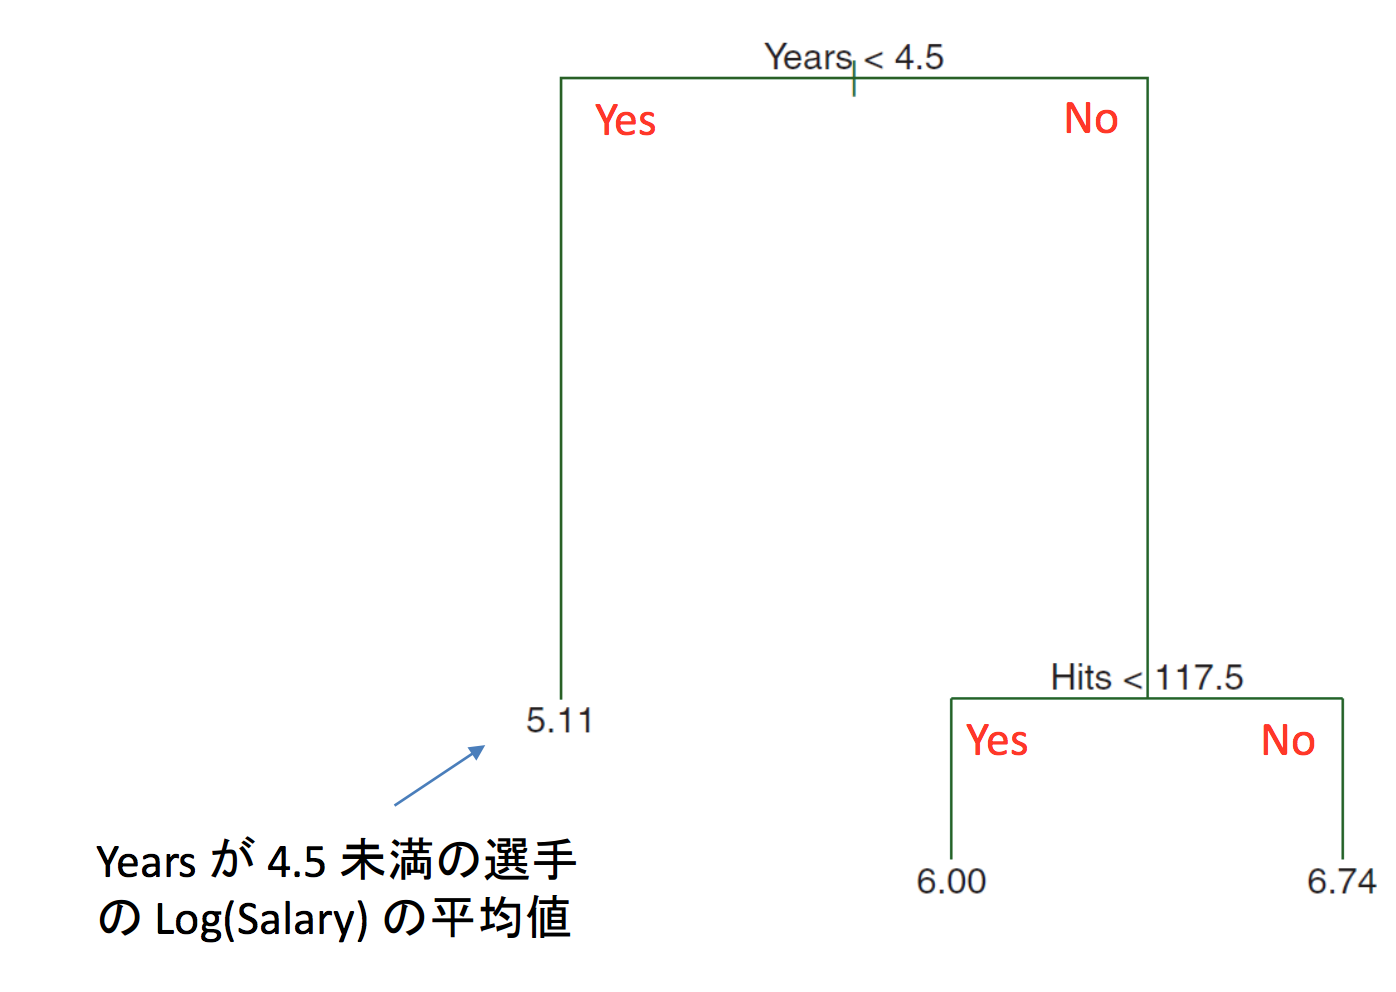
\includegraphics[width=70mm]{img/kaikiki.png}
 \end{center}
 \caption{Hittersデータに対する回帰木予測}
 \label{fig:one}
\end{minipage}
\begin{minipage}{0.5\hsize}
 \begin{center}
  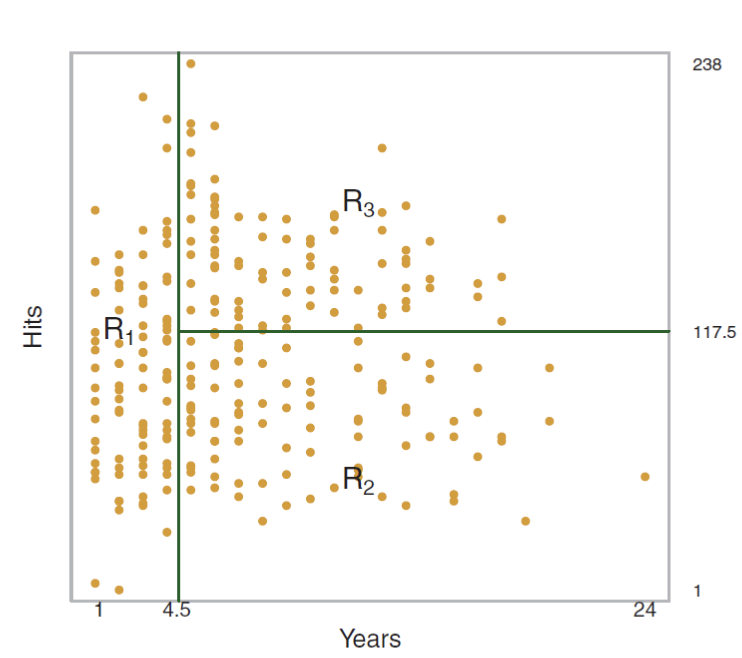
\includegraphics[width=70mm]{img/hitters.png}
 \end{center}
 \caption{Hittersデータに対する領域分割}
 \label{fig:two}
\end{minipage}
\end{figure}
回帰木の大まかの作り方は以下のようになります。
\begin{enumerate}
  \item 予測変数の空間を$J$個の領域$R_1, R_2, \ldots , R_j$に区分けをする。
  \item 予測変数の値が領域$R_j$に含まれる入力に対し、$R_j$に含まれる学習データの応答変数の平均値を出力する。
\end{enumerate}
予測変数の空間を$J$個の領域$R_1, R_2, \ldots , R_j$に区分ける方法として、${\rm RSS}$を最小化する区分けを考えうる全てのくみあわせを試すことは計算量的に難しいため、とりあえず今ある空間を全ての予測変数と分割の基準値の組み合わせを考え、\
学習データの正解ラベルとモデルによって予測された値の差分の二乗和が最小になるよっっっっそく変数と分割の基準値を見つける方法があります。
\begin{itembox}[l]{貪欲法による領域の分割}
  全ての予測変数$X_1, X_2, \dots, X_p$と分割の基準値sを組み合わせ、以下が最小になる分割方法を選択する。\
  $$\sum_{i:x_i \in R_1(j, s)} (y_i - \hat{y}_{R_i})^2 + \sum_{i:x_i \in R_2(j, s)} (y_i - \hat{y}_{R_2})^2$$
  $$ R_1(j, s) = \{X|X_j < s\}$$
  $$ R_2(j, s) = \{X|X_j \geq s\}$$
\end{itembox}
このような方法により分割された領域を示しているのが図10であり、$R_1, R_2, R_3$が終端ノード(つまり分類木ならこれが予測カテゴリに、回帰木ならこのリージョンに含まれたデータの平均値が予測結果となります)です。\
仮にYears $<$ 4.5以下の選手の事例が与えられれば彼は自動的に$R_1$に分類され、Years $> 4.5$かつ$Hits \leq 117.5$ならばこの事例は$R_2$に含まれることが分割図からもわかります。\
ただ、分割によって作られた二つの領域をさらに同様に分割し、領域に含まれる事例の数が閾値以下になるまで繰り返し再帰的に領域を構築していく\
こういった分割方法だと、領域同士が入り組んだ分割を行うことはでき図、複雑な分割には対応できない恐れがあります。
また、回帰木はデータに対して容易にオーバーフィットしてしまうため、枝刈りによって木のサイズを小さくして過学習を抑制する必要があります。
\begin{itembox}[l]{枝刈り}
  一旦木を構築してしまってから、Cost Complexity Pruningによって多すぎる枝分かれ(領域)を減らしていくこと。\
  $$\sum_{m=1}^{|T|}\sum_{i:x_i \in R_m} (y_i - \hat{y}_{Rm})^2 + \alpha|T|$$
  ここでTは木のノード数です。
\end{itembox}
Cost Complexity Pruningは、木のノードの数(すなわち枝分かれの数)に対してペナルティをつけて行き、ただ{\rm RSS}でフィットさせるのではなく、どこの枝同士をマージすべきかを計算して求めます。ここで$\alpha$は任意の値であり、\
$\alpha$を増やすと木は縮みます。このチューニングも縮小推定の$\lambda$のチューニングと同様、交差検証によって行います。\
% 実際にHittersデータでは、枝仮によってある程度エラーが。。。

\subsection{分類木}
分類木とは質的変数(カテゴリなど)を応答変数(予測したい値、$Y$)とし、末端ノードの出力は回帰木のような平均ではなく、多数決でラベルを決定する。\
分類木の構築は回帰木と同様、再帰的な分割を繰り返すことにより行います。しかしここで値を求める際の指標では分類誤り率(正しくカテゴリが予測されているか否か)ではなく、\
Gini indexやentropy等が用いられることが多いです。単なる正解率で考えないのは多数決により分類木のラベルを決定するため、単純な正解率によるモデル評価はこの多数決で少数派となったラベルについての情報が考慮されなくなってしまうためです。

\begin{itembox}[l]{Gini indeとentropy}
  $\hat{p}_{mk}$を領域$m$に含まれるクラス$k$の事例の割合とすると、
  \begin{description}
    \item [Gini index]\mbox{}\\
    $$G = \sum_{k=1}^K\hat{p}_{mk}(1 - \hat{p}_{mk})$$
    \item [entropy]\mbox{}\\
    $$D = -\sum_{k=1}^K \hat{p}_{mk}\log{\hat{p}_{mk}}$$
  \end{description}
\end{itembox}

% \begin{figure}
%   \begin{center}
%     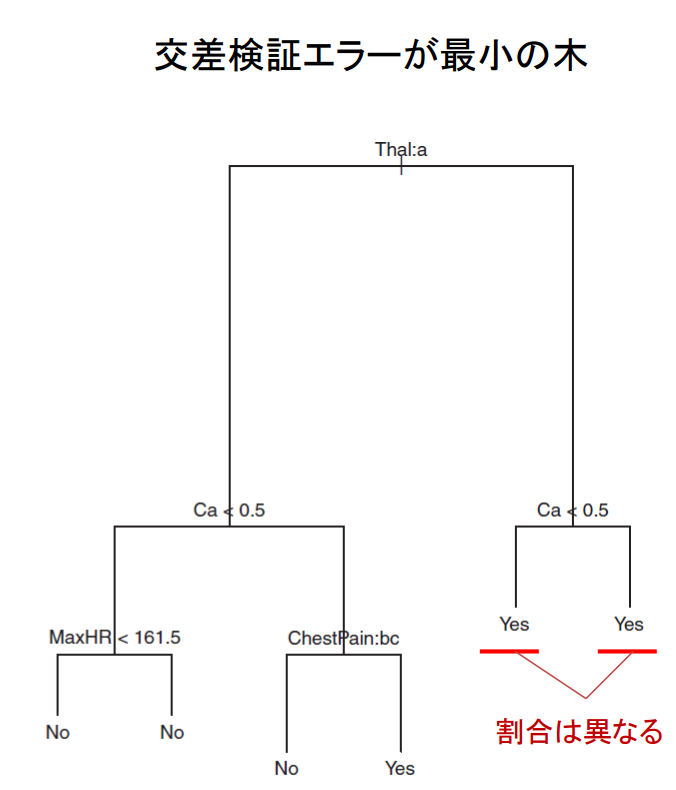
\includegraphics[width=8cm]{img/class_tree.png}
%     \caption{分類木予測}
%   \end{center}
% \end{figure}
枝刈りの結果、NOとNO、YESとYESに分岐するノードが存在するが、これは予測するクラスは同じではあるが、「どのくらいの確率でYES/NOか」が異なってくる。

\begin{figure}[htbp]
\begin{minipage}{0.7\hsize}
 \begin{center}
  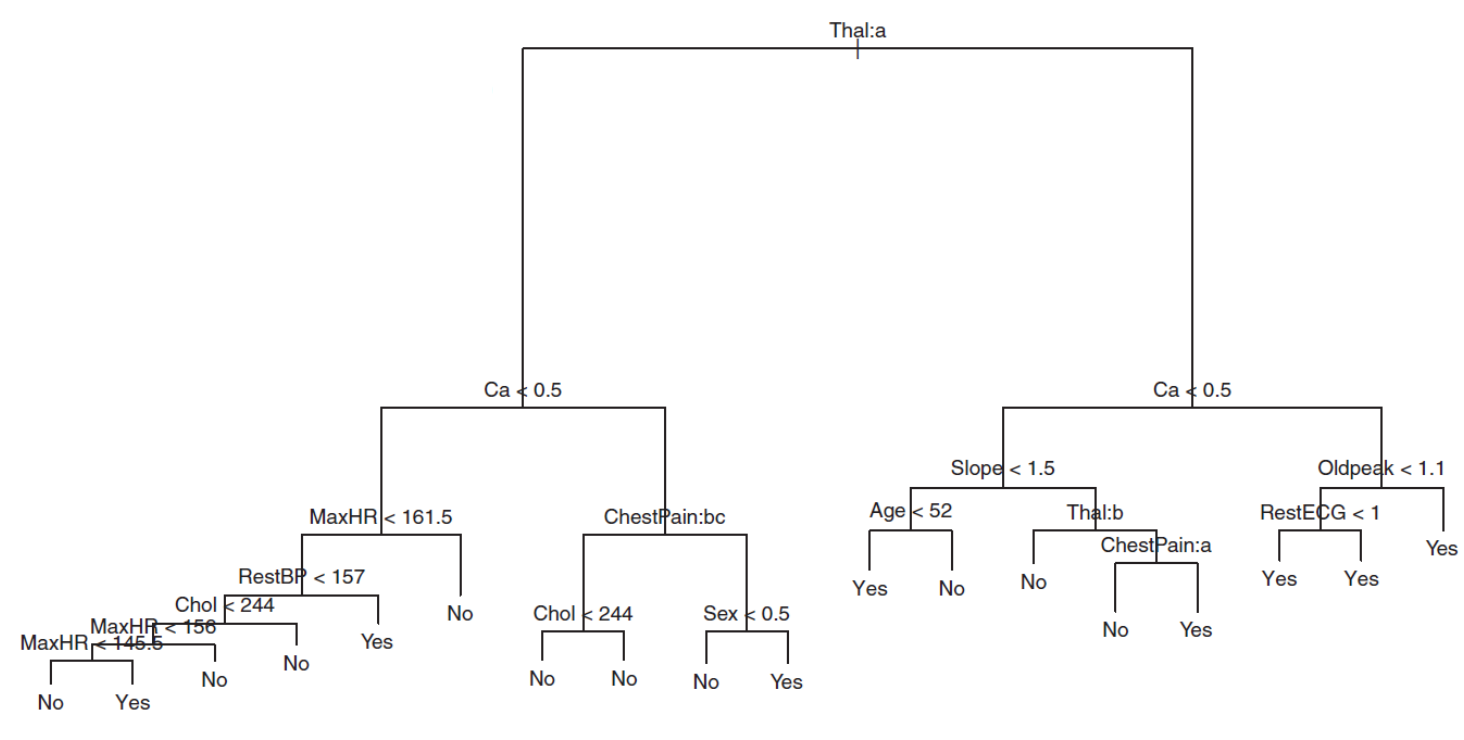
\includegraphics[width=100mm]{img/class_orig.png}
 \end{center}
 \caption{分類木によるHeartデータセット予測(枝刈り後)}
 \label{fig:one}
\end{minipage}
\begin{minipage}{0.3\hsize}
 \begin{center}
  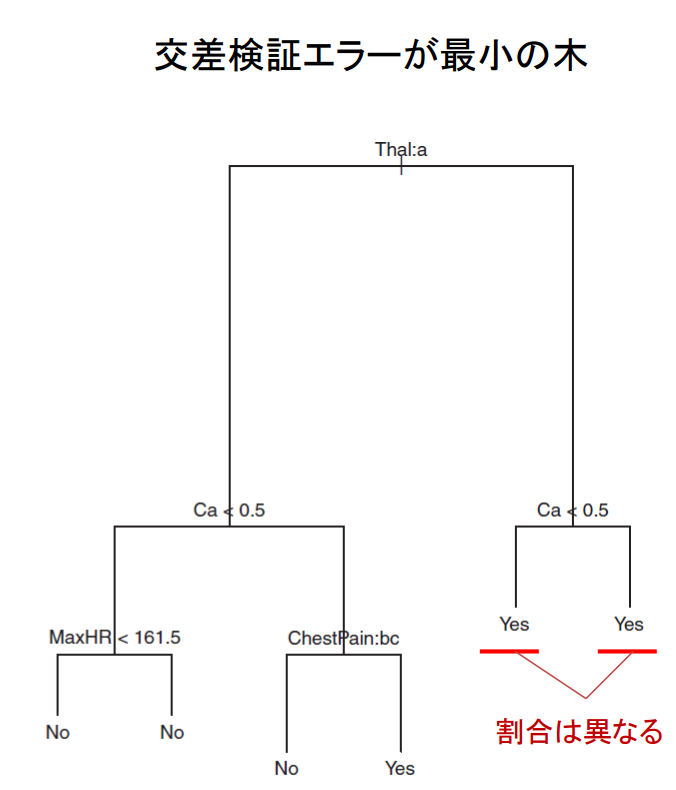
\includegraphics[width=50mm]{img/class_tree.png}
 \end{center}
 \caption{分類木によるHeartデータセット予測(枝刈り後)}
 \label{fig:two}
\end{minipage}
\end{figure}

\subsection{決定木の長所短所}
決定木の長所としては、以下の二点を上げることができます。
\begin{itemize}
  \item モデルが実際に利用した条件分岐などを確認でき、またそれも極めて人間の行う意思決定の方法に近いため学習結果の解釈が容易。
  \item 質的変数を扱う際にダミー変数を作らなくてよい
\end{itemize}
逆に短所としては
\begin{itemize}
  \item 回帰や分類の精度はあまり高くない(特殊なデータを除き、一般的な回帰モデル、分類モデルの方が高い精度を示すことが多い)
  \item 学習データにオーバーフィットしやすいため、学習データの小さな違いで構築される木が大きく変わることがある
\end{itemize}
例えば映画レビューをネガティブなものかポジティブなものか判断するとき、決定木モデルを用いるとある単語の有無で条件分岐を行うため、\
とてもネガティブな内容ではあるものの、学習データのポジティブなメールに多く含まれていた単語が多用されているレビューに対しては正しく予測できない可能性がより高くなる。\
ただ決定木はアンサンブル学習の「ランファムフォレスト」、ブースティング等により精度の向上が可能で、以下では以下に決定機による予測精度を向上するかについて説明します。

\subsection{バギング}
バギングはブートルトラップ(一つ抜き法によるサンプリング)によってバリアンス(異なる学習データ間での結果のばらつき。学習データによってフィットしすぎる結果、異なる学習データに対応できなくなる)を減らすことを目指す方法です。\
この出力は回帰木の出力の平均になります。Out-of-bag (OOB) エラー推定が便利です。複数の決定木の平均を取ることにより、個々の決定木よりも精度が高くなります。
\begin{itembox}[l]{バギング(bagging)}
  手順は以下の通りになる。
    \begin{enumerate}
      \item 学習データからn個の事例をランダムに復元抽出し、抽出された$n$個の事例を学習データとして決定木を構成する。
      \item これを$B$回繰り返す。
      \item 得られた$B$個の回帰木の出力の平均値が出力となる。分類木ならば平均を取る代わりに多数決で出力ラベルを決定する。
    \end{enumerate}
    $$\hat{f}_{bag}(x) = \frac{1}{B}\sum_{b=1}^B \hat{f}^{*b}(x)$$
\end{itembox}
また、バギングで用いられるエラー推定法をOut-of-bagエラー推定法といます。これはLOO交差検証とほぼ同等の推定結果を交差検証を行うことなく得られるので、\
効果的な推定法であると言えます。
\begin{itembox}[l]{Out-of-bag(OOB)エラー推定}
  OOB(Out-of-bag)とはブートストラップサンプルによって選択されなかったデータであり、\
  OOBエラー推定とは$B$個の回帰木に対して学習をさせた後、それぞれのOOBを用いて、OOBの中の$i$番目のデータと実際の結果$yi$を比較しテストを行い、\
  この誤り率(OOB推定値)をみる。
\end{itembox}

\subsection{ランダムフォレスト}
バギング$\footnote{この論文のランダムフォレストやブースティング、OOB、SVMの説明が結構わかりやすいです。時間のある方は読んでみてください。「ランダムフォレスト法による文章の書き手の同定」http://www.ism.ac.jp/editsec/toukei/pdf/55-2-255.pdf}$はシンプルにB個の決定木を構成し、その平均を取っているシンプルなモデルでした。これだけでも単一の決定木よりは精度が出るのですが、これをさらに改善した手法に「ランダムフォレスト」というモデルがあります。\
ランダムフォレストはそのシンプルかつ高い精度を実現するモデルでありSVM等と共に現実社会でも(割と)使われている機械学習モデルです。
\begin{itembox}[l]{ランダムフォレスト(random forest))}
  基本的な実行手順はバギングと同じ。ランダムフォレストでは、これに加えて決定木を構築するための再帰的な分割の際に考慮する予測変数を制限する。ランダムフォレストでは、各分割で考慮する予測変数をランダムに選択された$m$個の予測変数に限定する。$m = \sqrt{p}$がよく用いられる。
\end{itembox}
つまり、使用する入力変数を$m = p$としたランダムフォレストモデルはバギングと考えることもできます。あえて入力変数を減らした方が複数の決定木のアンサンブルにおいて精度が向上する理由としては、\
このように入力変数をランダムに選ぶことで、単純なバギングよりも構築される決定木のバリエーションが増え、構成された決定木の相関が減るためです。ちなみに分類の場合は$m = \sqrt{p}$が一般的ですが、回帰の場合は$m = p/3$が用いられることが多いらしいです。

バギングやランダムフォレストはシンプルな方法で精度を向上することが可能である一方、モデルの解釈が難しくなってしまう、またランダムフォレストの場合は分割によってRSSやGini Indexが減少してしまうという問題があります。
%
\subsection{ブースティング}
ブースティングとは、広義ではそこまで真の分類を精度高く予測できるわけではないモデル(弱学習器)を多数構築し、組み合わせることによりより高い精度をもつモデル(強学習器)を作ること意味します。
ここで組み合わされるモデルは決定木に限らず、様々なモデルに適用可能です。
\begin{itembox}[l]{ブースティング(boosting)}
  一連の弱学習器を多数構築し、まとめることで強学習器を構成し、性能を向上させること。
\end{itembox}
ブースティング自体は決定木に限定した内容ではないのですが、回帰木にブースティングを適用することにより、より性能の高いモデルを構成することができます。\
(ブースティングの手順のスライドがちょっとわかりにくいので多分後で補足します)

回帰木におけるブースティングでは、小さな回帰木を多数作り、構築されたモデルによる予測結果と実際のデータとの残差を応答変数として回帰木を作ります。最終的なモデルの出力は構築された多数の回帰木の出力の和になります。
\section{サポートベクターマシン(第12講)}
\subsection{サポートベクターマシンとは?}
サポートベクターマシンは元々二値分類$\footnote{クラスが二つの場合の分類問題}$のための識別モデルで、1990年代に開発されその高い精度から現在でも様々な場面で活用されています。\
一般的に「サポートベクターマシン」と総称することが多いのですが、
\begin{itemize}
  \item 最大マージン分類器 : マージンを最大化することによる分類。線形分離可能な場合以外は適応が難しい。
  \item サポートベクター分類器 : 線形分離可能でない場合でも適用可能だが、分離超平面は線形な関係に基づいている。
  \item サポートベクターマシン : カーネルにより非線形分類が可能であり線形分離の極めて難しい入り組んだデータでも対応は可能。
\end{itemize}
と実は細かく定義が分かれています$\footnote{実際に使用する場面ではほとんど区別していないと先生談}$。

\subsection{最大マージン分類器}
ある入力$X$がそのクラスに所属するかを超平面(hyperplane)により分割するものです$\footnote{ちなみにSVMは若干概念的にこれまでのモデルよりややこしく感じるかもしれません。この資料とかがわかりやすいかも。http://www.sakurai.comp.ae.keio.ac.jp/classes/infosem-class/2005/07SVM.pdf}$。\
超平面とは言ってはいますが、入力が二次元であれば直線、三次元であれば平面になります。
\begin{itembox}[l]{最大マージン分類器}
  $p$次元空間中の超平面とは、p-1次元の平坦な部分空間であり、以下の式で表される。
  $$\beta_0 + \beta_1X_1 + \beta_2X_2 + \ldots +\beta_pX_p = 0$$
  空間は超平面により超平面より大きいか小さいかにより、二つに区分される。
  \begin{numcases}
  {}
  \beta_0 + \beta_1X_1 + \beta_2X_2 + \ldots +\beta_pX_p > 0 & \\
  \beta_0 + \beta_1X_1 + \beta_2X_2 + \ldots +\beta_pX_p < 0 &
\end{numcases}
\end{itembox}
% 例えば、以下のような二次元空間中で、超平面を$1 + 2X_1 + 3X_2 =0$とすると、\
% 直線の上の青い部分が$1 + 2X_1 + 3X_2 > 0$
では、このような超平面はどのように求められるのでしょうか。まず、以下のような$n \times p$のデータ行列X、$n \times 1$のクラスラベル$y$から構成される学習データと、$1 \times p$で構成されるテストデータ$x^*$を考えます。\
つまり、$p$個の入力変数をもつ$n$個のデータとそれに対応した正解ラベルのペアを使って、新しい1個のテスト事例(同様に$p$個の入力変数を持つ)を正しく分類する分類器をこれから構築していくことを考えます。
\[
  X = \left(
    \begin{array}{cccc}
      x_{11} & x_{12} & \ldots & x_{1p} \\
      x_{21} & x_{22} & \ldots & x_{2p} \\
      \vdots & \vdots & \ddots & \vdots \\
      x_{n1} & x_{n2} & \ldots & x_{np}
    \end{array}
  \right)
\]
\[
 Y = \left(y_1\ y_2\ \dots\ y_n \right)^T \in \{-1, 1\}\
\]
\[
  \bm{x^*} = \left(
    \begin{array}{c}
      x_1^* \\
      x_2^*\\
      \vdots \\
      x_p^*
    \end{array}
  \right)
\]
\begin{itembox}[l]{分離超平面}
  学習事例をすべて正しく分類する超平面を最大マージン分類器における分離超平面という。
  \begin{numcases}
  {}
  \beta_0 + \beta_1X_1 + \beta_2X_2 + \ldots +\beta_pX_p > 0 \ {\rm if}\  y_i = 1& \\
  \beta_0 + \beta_1X_1 + \beta_2X_2 + \ldots +\beta_pX_p < 0 \ {\rm if}\  y_i = -1 &
\end{numcases}
より、全てのiに対して$y_i(\beta_0 + \beta_1x_{i2} + \ldots \beta_px_{ip}) >0$が成立し、テスト事例の分類は$x^*$をこの分離超平面に代入した時の正負により行えれる。

\end{itembox}
% \begin{description}
%   \item[分離超平面]\mbox{}\\
%   $n$個の学習事例すべてを正しく分類する超平面
% \end{description}
とりあえず全ての学習事例を正しく分類できてれば良いため、分離超平面は無数に存在しうることになります。ただ学習事例を分離可能な複数な超平面の中にも、\
少しノイズが入っただけで誤った分類をしてしまいそうな危うい超平面よりは、どちらのクラスよりもある程度離れている(つまり超平面が入力データのギリギリに惹かれているわけではない)超平面を選んだ方が、\
新たな入力に対しても頑健なモデルになりそうです。

最も近い学習事例までの距離をマージン、超平面に最も近い事例をサポートベクターと言います。最大マージン分類器は、このマージンを最大にすることにより、様々な入力に対して適切に分類を行うことのできるモデルの構築を目指しています。
\begin{itembox}[l]{最大マージン分類器の構築}
  学習事例を$x_1, \ldots x_n$、それに対応したクラスラベル$y_1 \ldots y_n$の最大マージン超平面は以下の最適化問題をとくことにより求められる。
  \begin{equation*}
    \begin{aligned}
    & \underset{\beta_0, \beta_1, \ldots , \beta_p}{\text{Maximize\ M}} \\
    % & &\displaystyle{M}  \\
    & \text{subject to}\  \sum_{j=1}^p \beta_j^2 = 1 \\
    & y_i(\beta_0 + \beta_1x_{i2} + \ldots \beta_px_{ip}) \geq M \forall i = 1, \dots, n
    \end{aligned}
  \end{equation*}
\end{itembox}
つまり、$\sum_{j=1}^p \beta_j^2 = 1$の時、$y_i(\beta_0 + \beta_1x_{i2} + \ldots \beta_px_{ip})$は超平面への距離を表しているため、全ての事例のうちこれが最も小さくなる事例(サポートベクター)におけるマージン$M$を最大にすることにより、超平面を求めています。
(なぜこれで超平面までの距離を表すことができるかはスライドを参照してください。)

最大マージン分類器は以下のような問題点があります。
\begin{itemize}
  \item そもそもデータが入り組んでおり、分離超平面を作ることができない\
  \item 分離超平面があった場合でも、学習データの変化に対して敏感に反応してしまうため、与えるデータによって大きく異なるモデルとなってしまう
\end{itemize}

\subsection{サポートベクター分類器の構築}
こういった最大マージン分類器の問題に対応することを目指しているのがサポートベクターマシンであり、マージンが小さく、設定されたマージンの内側に入ってしまうような事例や正しく判別されない事例を許容することで、データに大きく左右されないより頑健な$\footnote{余談ですがこういった入力データにいちいち左右されない頑健なモデルのことをロバスト(robust)なモデルと言います}$モデルを構築することを目指しています。
\begin{itembox}[l]{サポートベクター分類器}
  \begin{equation*}
    \begin{aligned}
    & \underset{\beta_0, \beta_1, \ldots , \beta_p, \varepsilon_1, \dots , \varepsilon_n}{\text{Maximize\ M}}\\
    % & \displaystyle{M}  \\
    & \text{subject to}\ \sum_{j=1}^p \beta_j^2 = 1 \\
    & y_i(\beta_0 + \beta_1x_{i2} + \ldots \beta_px_{ip}) \geq M(1 - \varepsilon_i) \forall i = 1, \dots, n \\
    & \varepsilon_i \geq 0,\ \sum_{i=1}^n \varepsilon_i \leq C
    \end{aligned}
  \end{equation*}
\end{itembox}
$\varepsilon$をスラック変数といい、$\varepsilon = 0$ならば違反を許さず、この分類器は上述の最大マージン分類器と同地になりますが、$\varepsilon > 0$ならば、ある事例がマージン$M$より$\varepsilon$分だけ分離超平面に\
接近していることを許すため、マージンの制約に違反していることがわかります。また、$\varepsilon > 1$、例えば$\varepsilon$を2に設定すると、$1 - \varepsilon = 1 - 2 = -1$となり、クラスAに分類されるはずの事例が超平面の向こう側(つまりクラスB)に分類されることを許容していることになります。\
つまり$\varepsilon$を大きくすることでより許容度を上げていくことができるのですが、全て許容していてては逆に全く正しくない超平面となってしまうためある定数$C$に制限し、違反を合計でどれだけ許すかを定めます。
$C$の値は交差検証等で適切な値を探すことが多いのですが、この大小はモデルに対して以下のような影響を与えます。
\begin{description}
  \item[$C$の値が大きい時]\mbox{}\\
  \begin{itemize}
    \item $C$を大きくすると、超平面の反対側やマージンの内側に事例が存在することが多くなるため、サポートベクターの数が多くなる。
    \item 入力事例の変化には頑健になるためバリアンスは小さくできるが、バイアスは大きくなってしまう。
  \end{itemize}
  \item[$C$の値が小さい時]\mbox{}\\
  \begin{itemize}
    \item $C$が小さければモデルはより最大マージン分類器に近くなりサポートベクターの数は少なくなる。
    \item $C$が小さいと入力される事例の変化によって超平面がどんどん動くので、バリアンスは大きいが、今あるデータにはよくフィットするためバイアスは小さくなる。
  \end{itemize}
\end{description}
% $C$を大きくすると、超平面の反対側やマージンの内側に事例が存在することが多くなるため、サポートベクターの数が多くなります。一方、$C$が小さければモデルはより最大マージン分類器に近くなりサポートベクターの数は少なくなります。\
% また、$C$が大きいと、入力事例の変化には頑健になるためバリアンスは小さくできるが、バイアスは大きくなってしまう。このように、サポートベクター分類器では、境界が非線形性を持っていてもある程度分類が可能ではあるものの、\
% 境界自体は線形に引かれるため、非線形な境界を引くことには限界があり、そこで次のサポートベクターマシンは非線形な教会による分類を目指しています。

% また、LDAの場合では、分離面から大きく離れているような事例も結果に影響を与えていましたが、サポートベクターマシンではマージンの外側にあるような事例は結果に影響を与えません。\
ただサポートベクター分類器は許容度をあげてはいるものの、線形な境界に基づいた分類であるため完全に入り組んだ(螺旋状にデータが散らばっている等)の事例にはうまく対応ができません。次のサポートベクターマシンはこういったケースに対応するため非線形な境界による分類を可能にしています。
\subsection{サポートベクターマシン}
来週の授業で喋るっぽいので来週追加します。

\section{Rチートシート}

\section{参考資料}
授業で「参考」とされた内容や数式の計算過程等をまとめてあります。
\subsection{リッジ回帰、Lasso回帰を不等式制約付きの最適化問題として捉える}
リッジ回帰、Lasso回帰は以下のような不等式条件付きの最適化問題として捉えることができ、この見方をするとなぜLasso回帰においてパラメータが0に収束しやすいのか\
理解がしやすくなります。

\begin{itembox}[l]{不等式条件つき最適化問題としての等式化}
  \begin{description}
    \item[リッジ回帰]\mbox{}\\
    \begin{equation*}
      \begin{aligned}
      & \underset{\beta}{\text{minimize}}
      & &\displaystyle{\sum_{i=1}^n \left(y_i - \beta_0 - \sum_{j=1}^p \beta_jx_{ij}\right)^2 }  \\
      & \text{subject to}
      & & \lambda \sum_{j=1}^p \beta_j^2 \leq s
      \end{aligned}
    \end{equation*}
    \item[Lasso回帰]\mbox{}\\
      \begin{equation*}
        \begin{aligned}
        & \underset{\beta}{\text{minimize}}
        & &\displaystyle{\sum_{i=1}^n \left(y_i - \beta_0 - \sum_{j=1}^p \beta_jx_{ij}\right)^2 }  \\
        & \text{subject to}
        & & \lambda \sum_{j=1}^p |\beta_j| \leq s
        \end{aligned}
      \end{equation*}
  \end{description}
  %
  % 縮小推定別な表現の方法も
  % ゼロでない変数が最大s個という制約を加えることも可能。これはまずい〜ー>勾配を見ながらbetaを探しているw毛ではない、
  % 製薬の形で考えると、なぜらっそだとパラメータがゼロになるかがわかる
  % らっそだとダイヤモンドの中に入る必要。雪片あたりで{\rm RSS}の等高線と一致する
  % リッジ回帰は事情ノルムの制約がつく。ベータ1も2もゼロになることはない
  % Lasso v.s. リッジ
  % 問題によって変わります
\end{itembox}
\subsection{予測誤差の大きさ(第3講)}
予測結果$\hat{Y}$と実際のラベル$Y$の二乗誤差の期待値を計算してみる。
統計的機械学習において、$Y = f(X) + \epsilon$で表されるため、
$$E[(Y - \hat{Y})^2] = E[((f(X) + \epsilon) - \hat{f}(X))^2]$$

\subsection{Bias-variance trade-offの導出(第4講)}



\subsection{線形単回帰のパラメータの推定法(第4講)}
線形単回帰の{\rm RSS}を最小にする$\hat{\beta}_0, \hat{\beta}_1$は、ぞれぞれで{\rm RSS}を偏微分し、偏微分した結果を0にする$\hat{\beta}_0, \hat{\beta}_1$を\
連立方程式にとけば求めることができます。
$${\rm {\rm RSS}} = (y_1 - \hat{\beta_0} - \hat{\beta_1}x_1)^2 +  (y_2 - \hat{\beta_0} - \hat{\beta_1}x_2)^2 \ldots  (y_n - \hat{\beta_0} - \hat{\beta_1}x_n)^2$$
% (a + b + c)^2 = a^2 + b^2 + c^2 + 2ab + 2bc + 2ca
$$(y_1 - \hat{\beta_0} - \hat{\beta_1}x_1)^2 = y_1^2 + \hat{\beta_0}^2 + \hat{\beta_1}^2x_1^2 - 2y_1\hat{\beta_0} + 2\hat{\beta_0}\hat{\beta_1}x_1 -2\hat{\beta_1}x_1y_1より$$
% $$\frac{\partial {\rm RSS}}{\partial \hat{\beta_0}} = 0より$$
% $$\sum_{i=1}^n y_i - \beta_1\sum_{i=1}^n x_i - \beta_0 n = 0$$
% $$\frac{\partial {\rm RSS}}{\partial \hat{\beta_1}} = 0より$$
\begin{numcases}
  {}
  \frac{\partial {\rm RSS}}{\partial \hat{\beta_0}} = 0 \iff \sum_{i=1}^n y_i - \beta_1\sum_{i=1}^n x_i - \beta_0 n = 0  & \\
  \frac{\partial {\rm RSS}}{\partial \hat{\beta_1}} = 0 \iff \sum_{i=1}^n x_iy_i - \beta_1\sum_{i=1}^n x_i^2 - \beta_0 \sum_{i=1}^n x_i = 0  &
\end{numcases}
式(3)より
\begin{equation}
  \beta_0 = \frac{1}{n}\sum_{i=1}^n y_i - \beta_1\sum_{i=1^n}x_i
\end{equation}
ここで
\begin{equation}
  \overline{x} = \frac{1}{n}\sum_{i=1}^n x_i, \overline{y} = \frac{1}{n}\sum_{i=1}^n y_i
\end{equation}
式(5)(6)を式(4)に代入し、$\beta_1$について解くと、
\begin{equation*}
  \begin{split}
    \beta_1 &=  \frac{\sum_{i=1}^n x_iy_i - \frac{1}{n}(\sum_{i=1}^n y_i\sum_{i=1}^n x_i)}{\sum_{i=1}^n x_i^2 - \frac{\sum_{i=1}^n x_i^2}{n}} \\
    &= \frac{\sum_{i=1}^n(x - \overline{x})(y - \overline{y})}{\sum_{i=1}^n (x - \overline{x})^2}
  \end{split}
\end{equation*}
また式(5)より
$$\beta_0 = \overline{y} - \beta_1\overline{x}$$
\subsection{{\rm RSS}の性質の導出(第4講)}
式(5)について、全て一つのシグマでくくると
\begin{equation}
  \sum_{i=1}^n y_i - \beta_1x_i - \beta_0 = \sum_{i=1}^n e_i = 0
\end{equation}
よって、{\rm RSS}に関する一つ目の性質が示された。
また同様に式(6)より
\begin{equation}
  \sum_{i=1}^n x_iy_i - \beta_1x_i^2 - \beta_0 x_i = \sum_{i=1}^n x_i (y_i - \beta_1x_i - \beta_0)  =  \sum_{i=1}^n e_ix_i = 0
\end{equation}
よって二つ目の性質も{\rm RSS}からパラメータを推定する際に用いた式より導くことができる。

\subsection{標準誤差の求め方及び標準偏差(第4)}
母平均の信頼区間$ = 標本平均 \pm t \times 標本標準偏差 \div \sqrt{標本数}$です。
$$標準誤差 SE = \frac{標準偏差 SD}{\sqrt{標本数 N}}$$より、パラメータ$\beta_0, \beta_1$の信頼区間はそれぞれ
$$\hat{\beta}_0 \pm t{\rm SE}(\hat{\beta}_0), \hat{\beta}_1 \pm t{\rm SE}(\hat{\beta}_1)$$となる。
tの値はt分布表からtの値を求めることができる。信頼区間の当たる確率、すなわち95$\%$信頼区間であれば95$\%$を信頼係数といい、\
標本数から1を引いた数を自由度と呼び、t分布表ではこの自由度と信頼係数よりtの値を求めることができます。\
例えば標本数が10で95$\%$信頼区間を求めたい時、以下の表よりtは自由度が9、信頼係数が95$\%$の2.262ですことがわかる。\
標本数が大きくなるとこのtの値はほぼ正規分布の値と変わらず2前後になるため、線形単回帰のパラメータの信頼区間の推定において近似的に$t=2$とすることができる。
(ザックりな説明ですみません… https://blog.apar.jp/data-analysis/4632/)
\begin{figure}
  \begin{center}
  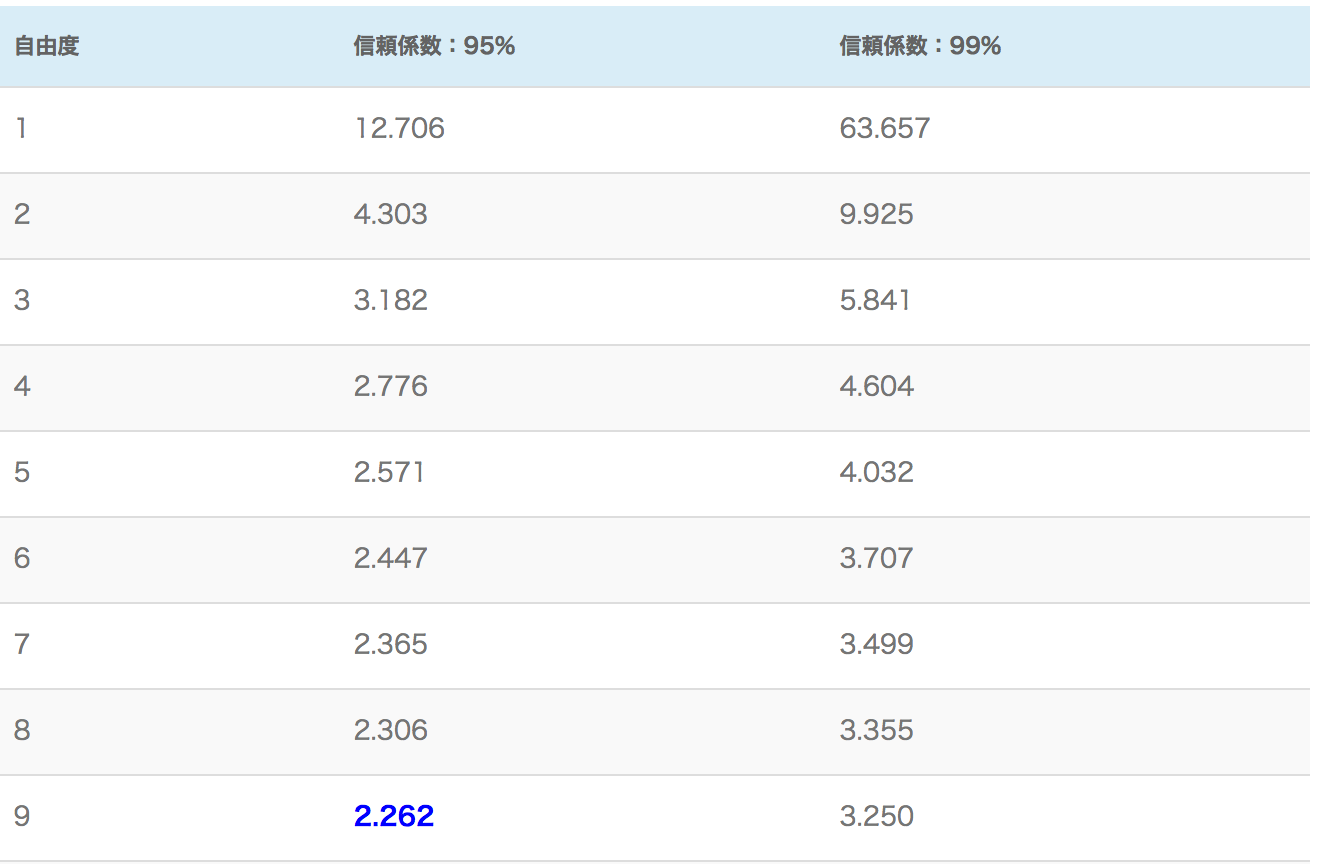
\includegraphics[width=10cm]{img/t_bunpu.png}
  \caption{t分布表の見方}
\end{center}
\end{figure}

\subsection{縮小推定の手計算(第10講)}
$n = p, \beta_0 = 0$
\[
  X = \left(
    \begin{array}{cccc}
      1 & 0 & \ldots & 0 \\
      0 & 1 & \ldots & 0 \\
      \vdots & \vdots & \ddots & \vdots \\
      0 & 0 & \ldots & 1
    \end{array}
  \right)
\]
という問題に対して、パラメータ推定及び縮小推定(リッジ推定、Lasso推定)を行う。

まず、最小二乗法でパラメータを推定する際には、
最小二乗法を用いる場合、その目的関数は以下のようになる。目的関数を最小化する$\beta_i$は目的関数の微分が0になる時となるため、
\begin{equation}
  L = \sum_{j = 1}^p(y_i - \beta_j)^2
\end{equation}
$$\frac{\partial L}{\partial \beta_i} = \frac{\partial}{\partial \beta_i}\sum_{j = 1}^p(y_i - \beta_j)^2 = \frac{\partial}{\partial \beta_i}(y_i^2 - 2y_i\beta_i + \beta_i^2) = -2(y_i - \beta_i)$$
$L$に対して$\beta_i$の微分を取る時、$i$番目以外のパラメータ$\beta$は無視してよいので、結果的に$L$を最小にする$\beta_i$の値は以下のようになる。

\begin{equation}
  \beta_i = y_i
\end{equation}

リッジ回帰においては目的関数が以下(5)で表現されるため、同様に$\beta_i$で微分をし、Lを最小化する$\beta_i$を求めると以下の(6)のようになる。
\begin{equation}
L = \sum_{i=1}^n \left(y_i - \beta_i \right)^2 + \lambda \sum_{j=1}^p \beta_j^2
\end{equation}

$$\frac{\partial L}{\partial \beta_i} = \frac{\partial}{\partial \beta_i}\left(\sum_{j = 1}^p(y_i - \beta_j)^2 +\lambda \sum_{j=1}^p \beta_j^2\right) + 2\lambda\beta_i = \frac{\partial}{\partial \beta_i}(y_i^2 - 2y_i\beta_i + \beta_i^2) = 2(1 + \beta_i) - 2y_i $$
\begin{equation}
  \hat{\beta_i^R} = \frac{y_i}{1 + \lambda}
\end{equation}
(6)より、$\lambda = 0$ならば目的関数を最小化する$\beta_i$がパラメータ推定の結果求められた(5)と一致することがわかり、\
$\lambda = 0$の縮小推定の結果はパラメータ推定により求められる値と一致することが確認できる。

Lasso回帰においては目的関数が以下(7)で表現される。Lasso回帰においては、正則化項が絶対値符号を含むため、$\beta_i$が正か負かで場合わけをする必要がある。
\begin{equation}
  L = \sum_{i=1}^n \left(y_i - \beta_i \right)^2 + \lambda \sum_{j=1}^p |\beta_j|
\end{equation}

% \begin{equation}
%   \frac{\partial L}{\partial \beta_i} = \frac{\partial}{\partial \beta_i}\left(\sum_{j = 1}^p(y_i - \beta_j)^2 +\lambda \sum_{j=1}^p \beta_j^2\right) + 2\lambda\beta_i = \frac{\partial}{\partial \beta_i}(y_i^2 - 2y_i\beta_i + \beta_i^2) = 2(1 + \beta_i) - 2y_i
%
% \end{equation}
















\end{document}
